% !TeX root = main_submission.tex

\documentclass[superscriptaddress,
               floatfix,
               longbibliography, 
               showkeys,apl]{revtex4-2}  
  
%\bibliographystyle{apsrevtitle}

\usepackage{graphicx} 
\usepackage{bm}	
\usepackage{color}                     
\usepackage{xcolor}
\usepackage{epsfig}
\usepackage{amsmath} 
\usepackage{amssymb} 
\usepackage{longtable} 
\usepackage{float}
\usepackage{mathtools}
\usepackage{dsfont}
\usepackage{xparse}
\usepackage{hyperref}
\usepackage{times}
\usepackage[normalem]{ulem}
\usepackage{sidecap}
\usepackage{appendix} 
\sidecaptionvpos{figure}{t}
\usepackage{comment}
\usepackage{physics}
\usepackage{float}
\usepackage{xfrac}
\newtheorem{theorem}{Theorem}
\usepackage{svg}
\usepackage{multirow}
\usepackage{algpseudocode}
\usepackage{tikz,lipsum,lmodern}
\usepackage[most]{tcolorbox}
\usepackage{tikz}

%% Text flags
\definecolor{darkgreen}{rgb}{0.0, 0.5, 0.0}
\newcommand{\wip}[2]{\textcolor{darkgreen}{[#1] #2}}

%\newcommand{\eg}{e.g.}
%\newcommand{\ie}{i.e.}

%PQC tasks
\newcommand{\ansatz}{\mathcal{U}} % Ansatz
\newcommand{\pqc}{\ansatz(\params)} % PQC

\newcommand{\objective}{C} % cost operator
\newcommand{\objectiveparams}{\objective(\params)} % cost operator

\newcommand{\costfunction}{\mathcal{C}} % PQC
\newcommand{\costfunctionstate}{\costfunction(\psi)} % PQC
\newcommand{\costoperator}{\mathcal{O}} % cost operator

\newcommand{\taskidx}{\tau} % cost operator
\newcommand{\taskidxtest}{\tau^{\prime}} % cost operator
\newcommand{\stateinit}{|\psi_0 \rangle} % cost operator
\newcommand{\statefinal}{|\psi(\params) \rangle}
\newcommand{\state}{|\psi \rangle}

\newcommand{\proj}[1]{|#1\rangle \langle #1|}


\newcommand{\be}{\begin{equation}}
\newcommand{\ee}{\end{equation}}
\newcommand{\bd}{\begin{displaymath}}
\newcommand{\ed}{\end{displaymath}}
\newcommand{\BE}{\begin{eqnarray}}
\newcommand{\EE}{\end{eqnarray}}
\newcommand{\vsp}{\vspace*{3mm}}
\newcommand{\pprime}{{\prime\prime}}
\newcommand{\R}{{\rm I\!R}}
\newcommand{\smallo}{{o}}
\newcommand{\plus}{{\!+\!}}
\newcommand{\minus}{{\!-\!}}
\newcommand{\sgn}{{\rm sgn}}
\newcommand{\erfc}{{\rm erfc}}
\newcommand{\id}{{\rm 1\!\!I}}
\newcommand{\ba}{\ensuremath{\mathbf{a}}}
\newcommand{\bb}{\ensuremath{\mathbf{b}}}
\newcommand{\bc}{\ensuremath{\mathbf{c}}}
\newcommand{\bh}{\ensuremath{\mathbf{h}}}
\newcommand{\bk}{\ensuremath{\mathbf{k}}}
\newcommand{\bq}{\ensuremath{\mathbf{q}}}
\newcommand{\bs}{\ensuremath{\mathbf{s}}}
\newcommand{\bu}{\ensuremath{\mathbf{u}}}
\newcommand{\bv}{\ensuremath{\mathbf{v}}}
\newcommand{\bw}{\ensuremath{\mathbf{w}}}
\newcommand{\bx}{\ensuremath{\mathbf{x}}}
\newcommand{\by}{\ensuremath{\mathbf{y}}}
\newcommand{\bz}{\ensuremath{\mathbf{z}}}
\newcommand{\bn}{\ensuremath{\mathbf{n}}}
\newcommand{\bolde}{\ensuremath{\mathbf{e}}}
\newcommand{\bee}{\ensuremath{\mathbf{e}}}
\newcommand{\boldeff}{\ensuremath{\mathbf{f}}}
\newcommand{\bA}{\ensuremath{\mathbf{A}}}
\newcommand{\bB}{\ensuremath{\mathbf{B}}}
\newcommand{\bC}{\ensuremath{\mathbf{C}}}
\newcommand{\bD}{\ensuremath{\mathbf{D}}}
\newcommand{\bF}{\ensuremath{\mathbf{F}}}
\newcommand{\bG}{\ensuremath{\mathbf{G}}}
\newcommand{\bGz}{\ensuremath{\mathbf{G_0}}}
\newcommand{\bRone}{\ensuremath{\mathbf{R_1}}}
\newcommand{\bJ}{\ensuremath{\mathbf{J}}}
\newcommand{\bK}{\ensuremath{\mathbf{K}}}
\newcommand{\bR}{\ensuremath{\mathbf{R}}}
\newcommand{\bT}{\ensuremath{\mathbf{T}}}
\newcommand{\bW}{\ensuremath{\mathbf{W}}}
\newcommand{\bM}{\ensuremath{\mathbf{M}}}
\newcommand{\bp}{\ensuremath{\mathbf{p}}}
\newcommand{\bCx}{\ensuremath{\mathbf{C_1}}}
\newcommand{\bCy}{\ensuremath{\mathbf{C_2}}}
\newcommand{\bGx}{\ensuremath{\mathbf{G_1}}}
\newcommand{\bGy}{\ensuremath{\mathbf{G_2}}}
\newcommand{\beff}{\ensuremath{\mathbf{f}}}
\newcommand{\hq}{\hat{q}}
\newcommand{\hw}{\hat{w}}
\newcommand{\hx}{\hat{x}}
\newcommand{\hy}{\hat{y}}
\newcommand{\hA}{\hat{A}}
\newcommand{\hC}{\hat{C}}
\newcommand{\hG}{\hat{G}}
\newcommand{\hK}{\hat{K}}
\newcommand{\hL}{\hat{L}}
\newcommand{\D}{{\cal{D}}}
\newcommand{\hbq}{\hat{\mbox{\boldmath{q}}}}
\newcommand{\qbo}{{\mbox{\boldmath{q}}}}
\newcommand{\hbx}{\hat{\mbox{\boldmath{x}}}}
\newcommand{\hbw}{\hat{\mbox{\boldmath{w}}}}
\newcommand{\hOmega}{\hat{\mbox{$\Omega$}}}
\newcommand{\bchi}{{\mbox{\boldmath{$\chi$}}}}
\newcommand{\boldeta}{{\mbox{\boldmath{$\eta$}}}}
\newcommand{\boldomega}{{\mbox{\boldmath{$\omega$}}}}
\newcommand{\boldpsi}{{\mbox{\boldmath{$\psi$}}}}
\newcommand{\boldphi}{{\mbox{\boldmath{$\varphi$}}}}
\newcommand{\bEta}{{\mbox{\boldmath{$\eta$}}}}
\newcommand{\bzeta}{{\mbox{\boldmath{$\zeta$}}}}
\newcommand{\boldOmega}{{\mbox{\boldmath{$\Omega$}}}}
\newcommand{\bxi}{\bm{\xi}}
\newcommand{\olx}{\overline{\mathbf{x}}}
\newcommand{\olxone}{\overline{x}_1}
\newcommand{\olxtwo}{\overline{x}_2}
\newcommand{\olxonedot}{\dot{\overline{x}}_1}
\newcommand{\olxtwodot}{\dot{\overline{x}}_2}
\newcommand{\bnull}{{\mbox{\boldmath{$0$}}}}
\newcommand{\rate}{\tilde{\eta}}
\newcommand{\double}{{\prime\prime}}
\newcommand{\tp}{t^\prime}
\newcommand{\td}{t^{\prime\prime}}
\newcommand{\wt}{\widetilde}
\newcommand{\avg}[1]{\left\langle{#1}\right\rangle}
\newcommand{\davg}[1]{\left\langle\left\langle{#1}\right\rangle\right\rangle}
\newcommand{\fE}{\mathbb{E}}
\newcommand{\ds}{\mathcal{D}\,\mathbf{S}}
\newcommand{\mcD}{\mathcal{D}}
\newcommand{\mcM}{\mathcal{M}}

\newcommand{\Jferro}{J_{\mathrm{F}}}


\newcommand{\Ham}[1]{H_{\mathrm{#1}}}
\newcommand{\Hnumfault}{\Ham{numfaults}}
\newcommand{\Hgate}{\Ham{gate}}
\newcommand{\Hfaultset}{\Ham{faultset}}
\newcommand{\Hconsist}{\Ham{consist}}
\newcommand{\Hmultfault}{\Ham{multfault}}
\newcommand{\weight}[1]{\lambda_{\mathrm{#1}}}
\newcommand{\faultweight}{\weight{faultset}}
\newcommand{\multfaultweight}{\weight{multfault}}
\newcommand{\gateweight}{\weight{gate}}
\newcommand{\OR}{\textsc{OR}}
\newcommand{\AND}{\textsc{AND}}
\newcommand{\XOR}{\textsc{XOR}}
\newcommand{\EQ}{\textsc{EQ}}
\newcommand{\BUFFER}{\textsc{BUFFER}}
\newcommand{\NOR}{\textsc{NOR}}
\newcommand{\NOT}{\textsc{NOT}}
\newcommand{\NAND}{\textsc{NAND}}

\renewcommand{\labelenumi}{(\roman{enumi})}
\newcommand{\expectedval}[1]{{\mathbb E}\left[ #1 \right]}
\newcommand{\probability}[1]{{\mathbb P}\left[ #1 \right]}


\DeclareMathOperator{\sign}{sign}
\DeclareMathOperator*{\argmin}{arg\,min}

\providecommand{\abs}[1]{\lvert#1\rvert}

\def\c#1{\textcolor{blue}{#1}}
\def\cc#1{\textcolor{red}{#1}}
\def\ccc#1{\textcolor{green}{#1}}

\newcommand{\fs}[1]{\textcolor{blue}{#1}}
\def\hs#1{\textcolor{magenta}{[#1]}}
\newcommand{\ws}[1]{\textcolor{orange}{#1}}
\newcommand{\pjl}[1]{\textcolor{darkgreen}{#1}}
\def\aak#1{\textcolor{orange}{[#1]}}
\def\apo#1{\textcolor{cyan}{#1}}
\def\apoNote#1{\textcolor{cyan}{\textbf{ [#1]} }}

\def\mm#1{\textcolor{green!10!orange!90!}{#1}}


%\NewDocumentCommand{\ceil}{s O{} m}{
%  \IfBooleanTF{#1} 
%    {\left\lceil#3\right\rceil} 
%    {#2\lceil#3#2\rceil} 
%}

\hyphenation{OptDigits}

\begin{document}


\title{Sparse Block-Encodings for Linear Combinations of Ladder Operators}


\date{\today} 

\ws{You can make comments}
\gus{using your shortcut}
\ks{and it'll put}
\ar{your comments}
\pjl{in your own color :D}

\begin{abstract}
\label{abstract}

In this work, we detail the construction of block-encodings for observables described as a linear combination of products of ladder operators acting on fermionic, antifermionic, and bosonic modes.
We refer to this constuction as LOBE (Ladder Operator Block-Encoding) and show how it can be used to simulate Hamiltonians involving interactions between these different types of particles.
Our work builds off of similar sparse block-encoding constructions for fermionic system, but generalizes them to include bosonic ladder operators.
Additionally, we establish a clear connection between these sparse block-encodings and LCU (Linear Combination of Unitaries) block-encodings.
This connection allows for implementations of these block-encodings that significantly reduce the rescaling factor of the block-encoding without significantly affecting the quantum resources required to implement the block-encoding.
Constructing efficient block-encodings that allow for interactions between fermions, antifermions, and bosons, paves the way for the simulation of systems that are not purely fermionic which is vital for the simulation of many models that arise in high-energy physics.

\end{abstract} 

\maketitle

\section{Glossary}
\label{sec:glossary}

Here we explicitly define the technical phrases and symbols used throughout this work:

\begin{itemize}
    \item \textit{term} ($T$): An operator defined as a product of ladder operators.
    \item $L$: The number of terms in the Hamiltonian.
    \item $\Omega$: The occupation cutoff for the bosonic modes. $\Omega$ gives the maximum number of bosons that can be present in a single mode. 
    \item $I$: The number of momentum modes. The subscripts $b$, $d$, and $a$ will be used to denote the number of modes for a particular particle type.
    \item $b_i$: Fermionic annihilation (creation - $b_i^\dagger$) operator acting on mode $i$.
    \item $d_i$: Antifermionic annihilation (creation - $d_i^\dagger$) operator acting on mode $i$.
    \item $a_i$: Bosonic annihilation (creation - $a_i^\dagger$) operator acting on mode $i$.
    \item $n_{i_b}$: The number of fermions ($b$) occupying the $i^{th}$ mode. $n_{i_d}$ and $n_{i_a}$ give the occupancy for antifermions and bosons respectively.
    \item $B_l$: The number of fermionic modes with ladder operators acting on them within the term $T_l$.
    \item $D_l$: The number of antifermionic modes with ladder operators acting on them within the term $T_l$.
    \item $B$: The maximum number of fermionic \& antifermionic modes with ladder operators acting on them within a single term ($\max{b_l + d_l}$).
    \item $A_l$: The number of bosonic ladder operators within the term $T_l$. Operators raised to an exponent ($p$) count as $p$ operators.
    \item $A$: The maximum number of bosonic ladder operators acting within a single term ($\max_l A_l$). 
    \item $M_l$: The number of bosonic modes with ladder operators acting on them within the term $T_l$.
    \item $M$: The maximum number of bosonic modes with ladder operators acting on them within a single term ($\max_l M_l$).
    \item $S_{l, i}$: The exponent of bosonic annihilation operators acting on the $i^{th}$ bosonic mode within the $l^{th}$ term.
    \item $R_{l, i}$: The exponent of bosonic creation operators acting on the $i^{th}$ bosonic mode within the $l^{th}$ term.
    \item \textit{"zeroed-out"}: When the coefficient of a state becomes zero.
    \item \textit{encoded subspace}: The chosen subspace of the ancilla qubits used in the block-encoding to denote where the non-unitary operator is stored. Typically, this is the subspace where all ancillae are in the $\ket{0}$ state.
\end{itemize}
\section{Introduction}
\label{sec:intro}

The simulation of many-body quantum systems is a promising potential application for quantum computers \cite{feynman2018simulating}.
Accessing the information of non-unitary operators - such as the Hamiltonian - within a quantum algorithm, which is comprised solely of unitary operations, is a necessary subroutine for performing such simulations.
This task has been pursued through various means, resulting in methods such as Trotterization \cite{suzuki1976generalized,hatano2005finding,lie1893theorie,trotter1959product,childs2021theory} and Block-Encoding \cite{lin2022lecture, poulin2018quantum, low2019hamiltonian}.

Block-Encoding describes a general strategy for encoding a non-unitary operator within a chosen subspace (block) of a larger unitary operator.
Two general frameworks for constructing block-encodings of different operators - sparse block-encodings \cite{berry2009black, childs2009universal, lin2022lecture} and Linear Combinations of Unitaries (LCU) \cite{childs2012hamiltonian} - have allowed for the exploration of explicitly compiled block-encodings of several systems.

Understanding the spacetime quantum resources - the number of qubits (space), the number of operations (time), and the rescaling factor (overhead) - required for quantum simulation algorithms is important for understanding the feasability of simulating different systems.
These quantum resource estimates are crucial as they allow us to gauge the practical usefulness of quantum computers, particularly those that have experimentally demonstrated quantum error correction \cite{bluvstein2024logical, acharya2024quantum}.

Many previous works have investigated the quantum simulation for purely fermionic systems, with a particular emphasis on the simulation of molecules in quantum chemistry \cite{aspuru2005simulated, peruzzo2014variational, babbush2014adiabatic, o2016scalable, babbush2018encoding, google2020hartree, lee2021even, kivlichan2020improved, campbell2021early}.
Another interesting set of quantum systems to simulate are those that are derived from quantum field theories \cite{Peskin:1995ev, jordan2012quantum} \ws{@Gus, pls add citation for all models (quartic, static, phi, yukawa)}, which have applications in areas such as high-energy physics \cite{bauer2023quantum}.
These systems often include interactions between fermions, antifermions, and bosons and several works have produced quantum resource estimates for simulating such systems \cite{camps2024explicit, liu2024efficient, rhodes2024exponential}.

In this work, we provide a novel framework for constructing block-encodings of second-quantized operators, which we refer to as Ladder-Operator Block-Encoding (LOBE).
This framework directly block-encodes operators comprised of creation and annihilation operators and does not require the use of operator transformations that expand fermionic \cite{jordan1928paulische, bravyi2002fermionic, seeley2012bravyi} and bosonic \cite{somma2005quantum} \ws{add standard binary citations} ladder operators in the Pauli operator basis.

We give numerical quantum resource estimates for implementing block-encodings of several classes of operators and several Hamiltonians that arise in quantum field theories.
This includes purely fermionic systems, purely bosonic systems, and systems which include fermions, antifermions, and bosons. 
We analyze the numerical spacetime quantum resources for LOBE - in comparison to techniques which require mapping ladder operators onto the Pauli basis - and find that LOBE results in constructions with better asymptotic scaling and lower numerical quantum resources for many of the systems examined.

This work is organized as follows.
In Section \ref{sec:theory}, we review the defined action of ladder operators on quantum states.
In Section \ref{sec:block-encoding}, we review block-encodings and discuss frameworks for constructing block-encodings of different operators.
In Section \ref{sec:ladder-op-oracles}, we describe the LOBE framework, show compiled block-encodings for several classes of second-quantized operators, and give analytical spacetime costs of the associated constructions.
In Section \ref{sec:results}, we provide numerical quantum resource estimates for block-encodings of various classes of operators and Hamiltonians.
In Section \ref{sec:conclusions}, we summarize the results presented in this work and discuss future directions.
Additionally, a glossary that defines the terminology and variables used throughout this work is given in Appendix \ref{sec:glossary}.

\section{Theory}

Give background of ladder operators and constructions of realistic Hamiltonians/Observables from ladder operators

\subsection{Encoding}
\label{subsec:encoding}

Here we'll discuss how we encode the physical states we are interested in terms of qubits/registers.

\ws{Question: do we want to also cost-out the unary encoding or just the "compact" encoding that we've been primarily working with?}

\subsection{Ladder Operators}
\label{subsec:operators}

\ws{@Gus, you probably have much better language to define all of this stuff. I just needed to write something down so I could reference it in the circuit construction. Don't hesitate to scrap anything in here.}


\subsubsection{Feromons and Antiferomons}

Define action of fermionic ladder operators.

Fermions (and antifermions) obey the Pauli-exclusion principle \ws{citation} and therefore the occupation of a (anti)fermionic mode can only be occupied ($\ket{1}$) or unoccupied ($\ket{0}$).
Fermionic (and antifermionic) ladder operators only act non-trivially on the qubits encoding the mode that the ladder operator acts on and we define their action as follows.

The fermionic creation operator is given by:
\begin{equation}
    b_i^\dagger \ket{n_{b_i}} = 
    \begin{cases} 
        (-1)^{\sum_{j < i} b_j} \ket{1}  & when \ket{n_{b_i}} is \ket{0} \\
        0 & when \ket{n_{b_i}} is \ket{1}
    \end{cases}
\end{equation}
where $b_i$ denotes a fermionic ladder operator on the $i^{th}$ mode, the $^\dagger$ indicates a creation operator, and $\ket{n_{b_i}}$ is the occupation of the $i^{th}$ fermionic mode.
An antifermionic creation operator is defined as above with the symbol $d$ to denote that the operator acts on antifermions.

For a fermionic creation operator, if the mode being acted upon is unoccupied, then the creation operator "creates" a fermion in that mode and applies a phase determined by the parity of the occupation of the previous modes.
Therefore the ordering of the modes in the encoding has an implication on the action of the operator that must be accounted for.
Since fermionic modes can only be either occupied or unoccupied, then if the mode is already occupied the operator zeroes the amplitude of the quantum state, thereby "destoying" that portion of the quantum state. 

The fermionic annihilation operator is given by:
\begin{equation}
    b_i \ket{n_{b_i}} = 
    \begin{cases} 
        (-1)^{\sum_{j < i} b_j} \ket{0}  & when \ket{n_{b_i}} = \ket{1} \\
        0 & when \ket{n_{b_i}} = \ket{0}
    \end{cases}
\end{equation}
and the antifermionic annihilation operator is likewise defined for $d$ instead of $b$.

The action of the annihilation operators is similar (and opposite) to the creation operators.
If the mode is already occupied, then the annihilation operator "annihilates" the fermion at that mode by setting the occupation to zero and applies a phase based on the parity of the occupation of the preceeding modes.
If the mode is unoccupied before the operator is applied, then the annihilation operator zeroes the amplitude.

\subsubsection{Bosos}

\begin{equation}
    a_i^\dagger \ket{n_{a_i}} = 
    \begin{cases} 
        \sqrt{n_{a_i} + 1} \ket{n_{a_i} + 1}  & when \ket{n_{a_i}} \neq \ket{\Omega} \\
        0 & when \ket{n_{a_i}} = \ket{\Omega}
    \end{cases}
\end{equation}
where $a_i$ denotes a bosonic ladder operator on the $i^{th}$ mode, the $^\dagger$ indicates a creation operator, $\ket{n_{a_i}}$ is the occupation of the $i^{th}$ bosonic mode, and $\Omega$ is the maximum allowable bosonic occupation.

\begin{equation}
    a_i \ket{n_{a_i}} = 
    \begin{cases} 
        \sqrt{n_{a_i}} \ket{n_{a_i} - 1}  & when \ket{n_{a_i}} \neq \ket{0} \\
        0 & when \ket{n_{a_i}} = \ket{0}
    \end{cases}
\end{equation}

\subsubsection{Commutation Rules}
\label{subsec:commutation}


\subsection{Observables}
\label{subsec:observables}

\subsubsection{Products of Ladder Operators (Terms)}

We define a \textit{term} ($T$) as a product of ladder operators that can act on fermionic, antifermionic, and bosonic modes:
\begin{equation}
    T = \prod_{m=0}^{M-1} c_m
\end{equation}
where $M$ is the number of ladder operators in the term and $c_m \in \{b_i, b_i^\dagger, d_i, d_i^\dagger, a_i, a_i^\dagger\}$.

The ladder operators ($c_m$) can be reordered arbitrarily with the introduction of additional terms due to the commutation rules described in \ref{subsec:commutation}.
In this work, we will have a preference for \textit{normal ordering} of the operators to obey the following structure:
\begin{equation}
    T = \Big( \prod_i (\delta_{b_i^\dagger} b_i^\dagger)(\delta_{b_i} b_i) \Big) \Big( \prod_i (\delta_{d_i^\dagger} d_i^\dagger)(\delta_{d_i} d_i) \Big) \Big( \prod_i (\delta_{a_i^\dagger} (a_i^\dagger)^r)(\delta_{a_i} (a_i)^s) \Big) 
\end{equation}
where $\delta$ takes the value $0$ or $1$ to denote if the operator is active in the term and the values $r$ and $s$ are positive integers $\in [0, \Omega]$ and denote the exponent of the bosonic ladder operators acting on that particular bosonic mode.

\ws{Describe number/occupation operators acting on fermions/antifermions and bosons and rewrite previous equation for $T$ including these operators.}

\subsubsection{Linear Combinations of Terms}

We can write Hamiltonians (or observables) in the form of linear combinations of terms:
\begin{equation}
    \label{eq:lclo}
    H = \sum_{l=0}^{L-1} \alpha_l T_l
\end{equation}
where $L$ is the total number of terms and $\alpha_l$ is a real-valued coefficient associated with the term $T_l$.
\section{Block-Encodings}
\label{sec:block-encoding}

Quantum algorithms are constructed as a series of unitary operators.
However, it is often necessary to access information regarding non-unitary operators within a quantum algorithm.
Block-Encoding refers to an access model to non-unitary operators wherein the information regarding the operator is stored in a marked subspace of a larger unitary operator.

If we let $H$ represent some Hermitian, non-unitary operator, then a block-encoding of $H$ is given by:
\begin{equation}
    U_H = 
    \begin{pmatrix}
    \bar{H} & * \\
    * & * 
    \end{pmatrix}
\end{equation}
where $U_H$ is the larger unitary operator, $\bar{H}$ is a rescaled form of the original operator such that all matrix elements have magnitude less than one, and matrix entries $*$ denote matrix elements that are chosen such that the $U_H$ is untiary.

The action of the block-encoding on an arbitrary quantum state ($\ket{\psi}$) can be defined as:
\begin{equation}
    \ket{\psi} \ket{0}_{\text{anc}} \rightarrow_{U_H} \bar{H} \ket{\psi} \ket{0}_{\text{anc}} + \beta \ket{junk} \ket{0_\perp}_{\text{anc}}
\end{equation}
where $\ket{}_{\text{anc}}$ is the ancilla register and $\beta$ is a complex coefficient that normalizes the quantum state.
In the above equation, the encoded subspace of $\bar{H}$ is chosen (without loss of generality) to be the all-zero state of the ancilla register.
The state $\ket{junk}$ represents the state of the system register outside of the encoded subspace and can typically be disregarded.

Measurement of the ancilla after the block-encoding is apply and post-selecting on the encoded subspace gives the success probably of applying the block-encoding.
This success probability is a function of the rescaling factor of $H / \bar{H}$ and can have important implication for the cost of algorithms constructed with block-encodings.  

\subsection{Linear Combination of Unitaries}
\label{subsec:lcu}

Linear Combination of Unitary (LCU) is a method for generating block-encodings of operators that can be written as:
\begin{equation}
    H = \sum_{l=0}^{L-1} \alpha_l U_l
\end{equation}
where $\alpha_l$ is some real-valued coefficient.

In this construction, the rescaled operator is given by:
\begin{equation}
    H = \lambda_{LCU} \bar{H}
\end{equation}
where the rescaling factor ($\lambda_{LCU}$) is the 1-norm of the coefficients of the unitary operators in the LCU:
\begin{equation}
    \lambda_{LCU} = \sum_{l=0}^{L-1} | \alpha_l |
\end{equation}

LCU is constructed via two oracles: \textit{Prepare} and \textit{Select}.
The action of the \textit{Prepare} oracle is to create a superposition state of an ancilla register that is weighted by the normalizes coefficients of the terms in the LCU when the ancilla register begins in the all-zero state.
We refer to this ancilla register as the \textit{index register} as it encodes the index of the term in the LCU.
This is given by:
\begin{equation}
    \ket{0^{\otimes \lceil \log_2 L \rceil}} \rightarrow_{Prepare} \sum_{l=0}^{L-1} \sqrt{| \bar{\alpha_l} |} \ket{l}
\end{equation}
where $\ket{l}$ is the computational basis state of the index register encoding the integer $l$ in binary and the noramlized coefficients are given by:
\begin{equation}
    \bar{\alpha_l} = \frac{\alpha_l}{\lambda_{LCU}}
\end{equation}

The action of the \textit{Select} oracle is to apply the unitary $U_l$ onto the system register \textit{controlled} on the index regsiter being in the state $\ket{l}$.
This is given by:
\begin{equation}
    Select: 
    \begin{cases} 
        Apply \hspace{0.125cm} U_l \hspace{0.125cm} on \hspace{0.125cm} \ket{\psi} & when \hspace{0.05cm} \ket{\text{anc}} \hspace{0.05cm} is \hspace{0.05cm} \ket{l} \\
        Undefined & Otherwise \\
    \end{cases}
\end{equation}

With these two oracles defined, a block-encoding of $H$ can be realized as:
\begin{equation}
    \begin{split}
        \ket{\psi} \ket{0}_{\text{\text{index}}} &\rightarrow_{Prepare} \ket{\psi} \sum_{l=0}^{L-1} \sqrt{| \bar{\alpha_l} |} \ket{l}_{\text{\text{index}}} \\
        &\rightarrow_{Select} \sum_{l=0}^{L-1} \big(\sqrt{| \bar{\alpha_l} |} (U_l \ket{\psi}) \ket{l}_{\text{\text{index}}} \big) + \beta^* \ket{\perp^*} \\
        &\rightarrow_{Prepare^\dagger}  \bar{H} \ket{\psi} \ket{0}_{\text{\text{index}}} + \beta \ket{\perp} \\
    \end{split}
\end{equation}
where $\ket{\perp}$ and $\ket{\perp^*}$ denote quantum states of both the system and the index register that are outside the encoded subspace.
The state within the encoded subspace, $\bar{H} \ket{\psi} \ket{0}_{\text{\text{index}}}$, gives the rescaled Hamiltonian applied to the quantum state.
\ws{The math on this is sketchy. Probably gonna replace this with something actually correct.}

\subsection{Sparse Block-Encoding of Pairing Hamiltonians}
\label{subsec:sparse-be}

An alternative framework for constructing block-encodings is the sparse oracle approach.
In this approach, we assume access to two oracles: $O_A$ and $O_C$.
$O_A$ performs a controlled-rotation of a signal qubit encoding the value of the matrix element \cite{lin2022lecture} \ws{Is there another citation for this?}.
On inputs $\ket{l}$ and $\ket{j}$, $O_C$ returns the row index of the $l^{th}$ nonzero element in column $j$ \cite{camps2024explicit}.
The general idea of these oracles is that $O_C$ indicates where the non-zero matrix elements are and $O_A$ encodes what the values of the corresponding matrix elements are. 

In \cite{camps2024explicit}, the authors provide circuit constructions for these two oracles for certain sparse matrices.
Liu et. al \cite{liu2024efficient} use this framework to construct a sparse block-encoding for a pairing Hamiltonian of the form:
\begin{equation}
    H = \sum_{ij}h_{ij}b^\dagger_i b_j
\end{equation}

\begin{figure}[h]
    \includegraphics[width=12cm]{figures/liu-construction.pdf}
    \caption{
        \textbf{Sparse Block-Encoding Circuit for Pairing Hamiltonians}
        A circuit diagram for the block-encoding described by Liu et. al \cite{liu2024efficient} is shown.
        The \textit{Diffusion} operator is implemented via \textit{Uniform State Preparation} (USP).
        The $O_A$ oracle is implemented by the series of $O_H^l$ operators (shaded in purple) which load the coefficients of the $l^{th}$ term.
        The $O_C$ oracle is implemented by the series of $U_l$ operators (shaded in orange) which apply the $l^{th}$ term onto the state.
    }
    \label{fig:liu-construction}
\end{figure}

The layout of these circuits is given in Figure \ref{fig:liu-construction}.
The \textit{USP} oracle in Figure \ref{fig:liu-construction} represents the \textit{Diffusion} operator of \cite{camps2024explicit} and \cite{liu2024efficient}.
This oracle creates an equal superposition of basis states from $\ket{0}\dots \ket{2^{\lceil \log_2{L} \rceil} - 1}$ on the index register where $L$ is the number of terms in the Hamiltonian.
We will elaborate on this operator in Subsection \ref{subsec:prepare}.

The sequence of $O_H^l$ operators implement the $O_A$ oracle.
This oracle performs a controlled rotation on an ancilla qubit that, given the basis state from the index register, rotates the ancilla qubit proportionally to the coefficient of the term.
Explicity, this is implemented via the following steps:
\begin{algorithmic}[1]
    \For{$\ket{l} \in [0, L-1]$}
        \If{$\ket{\text{index}} == \ket{l}$}
            \State $\ket{\text{anc}} \gets \ket{1}$
        \EndIf

        \If{$\ket{\text{anc}} == \ket{1}$}
            \State $\theta_l \gets 2\arccos(\alpha_l)$, where $\alpha_l$ is $h_{ij}$ and a predetermined ordering of $i$ and $j$ gives a function: $f(i, j) = l$.
            \State $\ket{0}_{\text{coeff}} \gets R_y(\theta_l) \ket{0}_{\text{coeff}}$ 
        \EndIf

        \State $\ket{\text{anc}} \gets \ket{0}$
    \EndFor
\end{algorithmic}
% \begin{enumerate}
%     \item Control on the index register being in the state $\ket{l}$ and store the quantum boolean in an ancilla qubit
%     \item Controlled on this ancilla, perform a Pauli-Y rotation on an additional ancilla of the angle $\theta_l = 2\arccos(\alpha_l)$, where $\alpha_l$ is the value of $h_{ij}$ where an ordering of $i$ and $j$ gives a function: $f(i, j) = l$
%     \item The "control" qubit is then reset to $\ket{0}$
% \end{enumerate}
where the ``for'' loop is a coherent for-loop implemented by a mulitplexor over the index register.
Additionally, $\ket{\text{anc}}$ is a clean ancilla qubit and $\ket{0}_{\text{coeff}}$ is a single qubit in a ``coefficient" register that begins in the $\ket{0}$ state on the branch of the wavefunction where $\ket{\text{anc}}$ is $\ket{1}$. 
A constraint on the coefficients $h_{i, j}$ is that they be scaled such that all have magnitude less than $1$ which can be easily achieved by rescaling the Hamiltonian by the maximum value of $h_{i, j}$ for all $i$ and $j$.

The $O_C$ oracle is constructed by the unitaries denoted as $U_0 \dots U_{L - 1}$. 
Each of the unitaries encodes the behavior of one term $T_l$ when acting on the system. 
In general, these unitaries are constructed with the following steps:
\begin{algorithmic}[1]
    \For{$\ket{l} \in [0, L-1]$}
        \If{$\ket{\text{index}} == \ket{l}$}
            \State $\ket{\text{anc}}_{\text{index}} \gets \ket{1}$
        \EndIf

        \If{$\ket{\text{anc}}_{\text{index}} == \ket{1}$ and $T_l \ket{\psi} \neq 0$ and $\ket{\text{valid}} == \ket{1}$}
            \State $\ket{\text{anc}}_{\text{ctrl}} \gets \ket{1}$
        \EndIf

        \If{$\ket{\text{anc}}_{\text{ctrl}} == \ket{1}$}
            \State $\ket{\psi} \gets T_l \ket{\psi}$
            \State $\ket{\text{valid}} \gets X \ket{\text{valid}}$
        \EndIf

        \State $\ket{\text{anc}}_{\text{ctrl}} \gets \ket{0}$
        \State $\ket{\text{anc}}_{\text{index}} \gets \ket{0}$
    \EndFor
\end{algorithmic}
% \begin{enumerate}
%     \item Control on the index register being in the state $\ket{l}$ and store the quantum boolean in an ancilla qubit
%     \item Control on the previous ancilla, the state of the subsystem that the term $T_l$ acts on nontrivially, and the validation qubit being in the state $\ket{1}$ and store the quantum boolean in an ancilla qubit. This "control" qubit now indicates if the current term should be applied onto the quantum state
%     \item A Fredkin gate swaps the occupations of the system register for $i \leftrightarrow j$. This is beecause $b^\dagger_i b_j \ket{\psi}$ is nonzero when $\ket{\psi}_i = \ket{0}$ \textit{and} $\ket{\psi}_j = \ket{1}$, in which after the term acts on $\ket{\psi}$, $\ket{\psi}_j$ and $\ket{\psi}_i$ will swap values,  \textit{or} when they are both $\ket{1}$, in which case, the operator becomes a number operator.
%     \item The "validation" qubit is set to $0$ to signify $H\ket{\psi}$ was performed.
%     \item The "control" qubit is then reset to $\ket{0}$
% \end{enumerate}
where $T_l$ in the case of the pairing Hamiltonian is performed by applying a Fredkin gate to swap occupations of the system register for $i \leftrightarrow j$.
This is because $b^\dagger_i b_j \ket{\psi}$ is nonzero when $\ket{\psi}_i = \ket{0}$ \textit{and} $\ket{\psi}_j = \ket{1}$, in which after the term acts on $\ket{\psi}$, $\ket{\psi}_j$ and $\ket{\psi}_i$ will swap values, \textit{or} when they are both $\ket{1}$, in which case, the operator becomes a number operator.
\ws{We need to clarify the bug in their construction.}

\subsection{Unification}
\label{subsec:unification}

Upon inspection of the two oracles constructed in \cite{liu2024efficient}, it can be seen that the sparse block-encoding they present can be constructed in the same framework as an LCU block-encoding, however, the terms in the linear combiation are not restricted to be unitary, but simply fermionic ladder operators.

The unitary operators comprising $O_H^l$ commute with both one another and the unitaries $U_l$. 
A more efficient ordering of these unitaries is to place $O_H^l$ directly before or after $U_l$.
In this construction, the multiplexor over the index register is only performed once and the quantum boolean determining the index can be used for both oracles:
\begin{algorithmic}[1]
    \For{$\ket{l} \in [0, L-1]$}
        \If{$\ket{\text{index}} == \ket{l}$}
            \State $\ket{\text{anc}}_{\text{index}} \gets \ket{1}$
        \EndIf

        \If{$\ket{\text{anc}}_{\text{index}} == \ket{1}$ and $T_l \ket{\psi} \neq 0$ and $\ket{\text{valid}} == \ket{1}$}
            \State $\ket{\text{anc}}_{\text{ctrl}} \gets \ket{1}$
        \EndIf

        \If{$\ket{\text{anc}}_{\text{ctrl}} == \ket{1}$}
            \State $\ket{\psi} \gets T_l \ket{\psi}$
            \State $\ket{\text{valid}} \gets X \ket{\text{valid}}$
        \EndIf

        \State $\ket{\text{anc}}_{\text{ctrl}} \gets \ket{0}$

        \If{$\ket{\text{anc}} == \ket{1}$}
            \State $\theta_l \gets 2\arccos(\alpha_l)$, where $\alpha_l$ is $h_{ij}$ and a predetermined ordering of $i$ and $j$ gives a function: $f(i, j) = l$.
            \State $\ket{0}_{\text{coeff}} \gets R_y(\theta_l) \ket{0}_{\text{coeff}}$ 
        \EndIf

        \State $\ket{\text{anc}}_{\text{index}} \gets \ket{0}$
    \EndFor
\end{algorithmic}
% \begin{enumerate}
%     \item Control on the index register being in the state $\ket{l}$ and store the quantum boolean in an ancilla qubit
%     \item Controlled on this ancilla, apply the term $T_l$ onto the system as described above
%     \item Controlled on this ancilla, perform a Pauli-Y rotation on an ancilla qubit of the angle $\theta_l = 2\arccos(\alpha_l)$
%     \item Uncompute the quantum boolean and proceed to the next value of $l$
% \end{enumerate}
This ordering significantly reduces the number of non-Clifford operations as the multiplexor over the index register is only performed once.

One can construct a block-encoding for a Hermitian operator written as and LCU using these steps wherein $T_l$ is the $l^{th}$ unitary in the LCU.
The main difference here with the circuit construction as compared to LCU is that the \textit{Prepare} oracle is not used to load the coefficients of the terms.
Instead, the coefficients of the terms are applied to a new ``coefficient'' register one-by-one immediately after the term $T_l$ is applied on the system.

The role of the rotation on the ``coeff'' qubit is to load the coefficient by rotating the shared quantum state of the system and the ancilla register into the encoded subspace such that the amplitude in the encoded subsapce is $\sqrt{| \alpha_l |}$.
As mentioned, this serves the same effective purpose as the \textit{Prepare} oracle in LCU.
We can replace both the $O_A$ oracle and the Diffusion oracles with calls to \textit{Prepare} as is done in LCU.
This results in a block-encoding of the form:
\begin{equation}
    U_{\text{Prepare}^\dagger} \big( \prod_{l=0}^{L-1} U_l \big) U_{\text{Prepare}} \ket{\psi} \ket{0}_{\text{anc}} = \bar{H} \ket{\psi} \ket{0}_{\text{anc}} + \beta \ket{\perp}
\end{equation}
where $\big( \prod_{l=0}^{L-1} U_l \big)$ is constructed as is done in \cite{camps2024explicit,liu2024efficient}.
This series of operators applying $U_l$ implements the \textit{Select} oracle, however, instead of applying unitary operators (as is done in LCU), it applies fermionic ladder operators onto the system.

In this construction, more rotations may be required as the \textit{Prepare} oracle is called twice.
In Section \ref{sec:results} we give numerical counts for the number of rotations and often find that the number of additional rotations is not significant.
The main advantage of this construction, as opposed to the use of the Diffusion operator and $O_A$, is that the rescaling factor is often significantly smaller.
The rescaling factor in this construction is the L1-norm of the coefficients whereas the rescaling factor of the sparse-oracle implementation is $2^{\lceil \log_2{L} \rceil} * \max{\alpha_l}$.
\ws{I believe the latter is a strict upper-bound of the former. This is probably obvious, but would be good to prove/show.}
In Subsection \ref{subsec:prepare}, these two methods and their effects on the rescaling factor are described in more detail.
In Subsection \ref{subsec:prepare}, we refer to the method using the Diffusion operator and $O_A$ as \textit{USP} and the method using the \textit{Prepare} oracle in LCU as \textit{ASP}.

\section{Ladder Operator Block-Encoding (LOBE)}
\label{sec:lobe}

In this section of the text, we'll do the following:
\subsection{Defining "Block-Encoding"}
\label{subsec:block-encoding}

\subsection{Prior Works}
\label{subsec:prior-works}

\subsubsection{Linear Combination of Unitaries}

\subsubsection{Sparse Block-Encoding of Pairing Hamiltonians}
stuff from Liu et al
\ws{Might ask you to fill this out @Gus}

\subsection{Rescaling of Coefficients Due to Bosonic Terms}
\label{subsec:rescaling}

The inclusion of bosonic ladder operators in our models requires rescaling the coefficients of our Hamiltonian such that they are always normalized and appropriately weighted.
As shown in Eqs. \ref{eq:bosonic-creation} and \ref{eq:bosonic-annihilation}, bosonic ladder operators acquire a coefficient on the state that is proportional to the square-root of the occupation of the state.
From these definitions, it is clear that if we were to apply a block-encoding that contains bosonic ladder operators onto a quantum state, the output quantum state may not be normalized.

To remedy this, we can rescale the coefficients that are picked up by the operators such that the states are always normalized.
In the case of bosonic ladder operators, we can rescale Eqs. \ref{eq:bosonic-creation} and \ref{eq:bosonic-annihilation} by dividing by the square-root of the maximum allowable occupation number plus one such that any coefficient acquired is $< 1$:
\begin{equation}
    \begin{split}
        a_i^\dagger \ket{n_{a_i}} &= \sqrt{\frac{n_{a_i} + 1}{\Omega + 1}} \ket{n_{a_i} + 1} \hspace{1em} when \ket{n_{a_i}} \neq \ket{\Omega} \\
        a_i  \ket{n_{a_i}} &= \sqrt{\frac{n_{a_i}}{\Omega + 1}} \ket{n_{a_i} - 1} \hspace{1.7em} when \ket{n_{a_i}} \neq \ket{0}
    \end{split}
\end{equation}
We do not redefine these equations for the cases where the state is annihilated since they will be the same as in Eqs.  \ref{eq:bosonic-creation} and \ref{eq:bosonic-annihilation}
These rescaled coefficients will be accounted for within the action of the $Select$ oracle as described in Subsubsection \ref{subsubsec:select}.

Since multiple bosonic operators may be present within a single term ($T_l$), then the overall coefficient of the output state will be rescaled by a factor of:
\begin{equation}
    \lambda_{k_l} = (\Omega + 1)^{k_l/2}
\end{equation}
where $k_l$ is the number of bosonic operators included in the term $T_l$.

Different terms within the Hamiltonian may have different numbers of bosonic operators and therefore will have differing rescaling coefficients of $\lambda_{k_l}$.
In order to guarantee that this rescaling is consistent across the different terms, we can classically preprocess the coefficients in the Hamiltonian such that after the block-encoding is applied, all output states have the same bosonic rescaling factor.
If we define $K \equiv \max_l{k_l}$, then we can define the preprocessed coeffieints as:
\begin{equation}
    \alpha_l \rightarrow \frac{\alpha_l}{(\Omega + 1)^{(K - k_l)/2}} \equiv \alpha_l^*
\end{equation}
where the coefficients $\alpha_l^*$ are the rescaled coefficients of the terms.

This preprocessing means that after the block-encoding is applied, all output states will be rescaled by a coefficient of $(\Omega + 1)^{(K)/2}$.
Therefore, the rescaled Hamiltonian that we block-encode is given by:
\begin{equation}
    H^* = \frac{H}{(\Omega + 1)^{K/2}}
\end{equation}
where $H^*$ is the rescaled Hamiltonian.

\subsection{Circuit Construction}
\label{subsec:circuit}

\begin{figure}
    \centering
    \includegraphics[width=8cm]{figures/lobe-block-encoding.pdf}
    \caption{\textbf{Ladder Operator Block-Encoding.}
    }
    \label{fig:lobe}
\end{figure}

In Figure \ref{fig:lobe}, we define the LOBE circuit in terms of generic oracles.
Disregarding the (optional) control qubit ($\ket{\textit{ctrl}}$), the LOBE circuit makes use of 5 qubit registers: $\ket{\textit{index}}$, $\ket{\textit{valid}}$, $\ket{\textit{coeff}}$, $\ket{\psi}$, and $\ket{0^{\otimes \alpha}}$.

The register denoted $\ket{\textit{index}}$ is referred to as the index register and is used to index the terms in the Hamiltonian as is done in LCU constructions. 
The integer representations of the computational basis states of the index register corresponds to the indices $l$ in Eq. \ref{eq:lclo}. 

The register denoted $\ket{\textit{valid}}$ consists of a single qubit and is referred to as the validation qubit.
It serves the same purpose as in \cite{liu2024efficient} which is to denote whether or not the term at the current index ($T_l$) will annihilate the quantum state.
If the term will annihilate the state, then the validation qubit remains in the $\ket{1}$ state such that the branch of the wavefunction stays outside the desired subspace of the block-encoding.
If the term will not annihilate the state, then the validation qubit gets flipped to the $\ket{0}$ state for the term $T_l$.

The register denoted $\ket{\textit{coeff}}$ is referred to as the coefficient register and is used to apply the coefficients associate with the term $T_l$. 
These coefficients include both the coefficients of the terms in the linear combination ($\alpha_l$) as well as the coefficients associated with the bosonic ladder operators.
One qubit is used to apply the $\alpha_l$ coefficient while a separate qubit will be required for each bosonic operator (defined as a creation, annihilation, or occupation operator acting with a positive integer-valued exponent) in the term.

The register denoted $\ket{\psi}$ is referred to as the system register and is used to encode the state of the system.
This register can be broken up into three subsequent registers: the fermionic system $\ket{\psi_b}$, the antifermionic system ($\ket{\psi_d}$), and the bosonic system ($\ket{\psi_a}$).
The encoding studied in this work is outlined in more detail in Subsection \ref{subsec:encoding}.

Finally, the register denoted $\ket{0^{\otimes \alpha}}$ is referred to as the clean ancillae register.
This register includes ancillae qubits that are promised to begin in the $\ket{0}$ state and are returned to this state at the end of the block-encoding circuit.

The LOBE circuit is structured similarly to an LCU circuit in that it involves sequential application of a $\textit{Prepare}$ oracle, a $\textit{Select}$ oracle, and then uncomputing the $\textit{Prepare}$ oracle using the daggered circuit.
In addition to these oracles, a single $X$ gate is applied to the $\ket{\textit{valid}}$ qubit in order to prepare this qubit in the $\ket{1}$ state.
This single $X$ gate is \textit{not} repeated on subsequent applications of the block-encoding.

\subsubsection{Prepare Oracle}
The $\textit{Prepare}$ oracle is applied to the index register to prepare a superposition over the computational basis states of this register.

\textbf{Uniform State Preparation}

The simplest implementation of the $\textit{Prepare}$ oracle is to prepare a uniform superposition over the computational basis states using a series of Hadamard gates on each qubit in the register.
The rescaling condition for this implementation is that the coefficients must be rescaled such that they all have magnitude $\leq 1$.
Let the largest coefficient magnitude be given by $\alpha^* = \max{|\alpha_l|}$.
Then, this rescaling imposes a constant rescaling factor of $\alpha^*$ and we refer to these rescaled coeffifients as $\Tilde{\alpha_l}$.
An additional rescaling factor of $2^{\lceil \log_2{L} \rceil}$ from the uniform superposition results in an overall rescaling of the Hamiltonian by a constant factor of:
\begin{equation}
    \lambda_{usp} = 2^{\lceil \log_2{L} \rceil} \alpha^*
\end{equation}
such that the rescaled Hamiltonian is given by:
\begin{equation}
    \bar{H} = \frac{H^*}{\lambda_{usp}}
\end{equation}

The quantum resource requirements of this implementation of $\textit{Prepare}$ are negligible as no ancillae are required and only Clifford operations (Hadamards) are performed.
However, this implementation of $\textit{Prepare}$ requires that the rescaled coefficients of the terms ($\Tilde{\alpha_l}$) be incorporated within the $\textit{Select}$ oracle which will be described in Subsubsection \ref{subsubsec:select}.

\textbf{Arbitrary State Preparation}

An alternative implementation of $\textit{Prepare}$ is to use the same implementation traditionally used in LCU circuits.
The coefficients are first rescaled by their $L1-norm$:
\begin{equation}
    \lambda_{asp} = \sum_{l=0}^{L-1} |\alpha_l|
\end{equation}
and the rescaled Hamiltonian is given by:
\begin{equation}
    \bar{H} = \frac{H^*}{\lambda_{asp}}
\end{equation}

It should be noted that $\lambda_{asp} \leq \lambda_{usp}$ \ws{with equality when the coefficients of the terms all have equal magnitude (confirm this)} \ws{and give some analytical proof for this bound}.

Then, a state preparation routine is applied that performs the following operation:
\begin{equation}
    \ket{0^{\otimes \lceil \log_2{L} \rceil}} \rightarrow_{\textit{Prepare}} \sum_{l = 0}^{L-1} \sqrt{|\alpha_l| / \lambda_{asp}} \ket{l}
\end{equation}
This results in a weighted superposition over the computational basis states where the squared amplitudes of the basis states are equal to the magnitude of the associated coefficients.

For Hamiltonians that have structure among the coefficients of the terms, implementations of the $\textit{Prepare}$ oracle can be constructed that leverage this structure.
In certain cases, this can drastically reduce the cost of $\textit{Prepare}$ such as is done for the Fermi-Hubbard model in \cite{babbush2018encoding}.
However, when a certain structure cannot be assumed, the Grover-Rudolph algorithm from \cite{grover2002creating} gives a formulaic routine to generate these $\textit{Prepare}$ circuits.

Gover-Rudolph requires $L-1$ rotations, with $1$ being uncontrolled and the others controlled.
The total number of left-elbows is given by:
\begin{equation}
    N_{\textit{left-elbow}} = L + 1 
\end{equation}
with an equal number of right-elbows.
The total number of ancillae is given by:
\begin{equation}
    Q_{asp} = \lceil \log_2{L} \rceil - 2
\end{equation}
It should be noted that these ancillae, which will be returned to $\ket{0}$ after the oracle call completes, will likely be reused in the $\textit{Select}$ oracle and therefore will not contribute to the total qubit requirement of the block-encoding.

Overall, after the bosonic coefficient rescaling is applied and one of these $Prepare$ oracle compilations is chosen and the coefficients rescaled again, the overall rescaling of the Hamiltonian that is block-encoded is given by:
\begin{equation}
    \bar{H} = \frac{H}{(\Omega + 1)^{K/2} \lambda}
\end{equation}
with $\lambda$ being either $\lambda_{usp}$ or $\lambda_{asp}$.

\subsubsection{Select Oracle}
\label{subsubsec:select}


\begin{figure}
    \centering
    \includegraphics[width=16cm]{figures/select-broad.pdf}
    \caption{\textbf{Ladder Operator Select Oracle.}
    }
    \label{fig:select-broad}
\end{figure}

\begin{figure}
    \centering
    \includegraphics[width=16cm]{figures/select-specific.pdf}
    \caption{\textbf{Ladder Operator Select Oracle.}
    }
    \label{fig:select-specific}
\end{figure}

The $Select$ oracle is shown in Figure \ref{fig:lobe} as the oracle within the blue shaded region.
As is done in standard LCU circuits, the $Select$ oracle is designed such that it applies the term $T_l$ onto the system when the index register is in the computational basis state $\ket{l}$.
In Figure \ref{fig:lobe}, the hexagonal box represents the multiplexing operation given in Figure 7 of \cite{babbush2018encoding} which creates a coherent for-loop over the computational basis states using $L - 1$ left-elbows and $\lceil \log_2{L} \rceil$ ancillae qubits.

In Figure \ref{fig:select-broad}, we depict a broad schematic for applying a single term within the $Select$ oracle in LOBE and in Figure \ref{fig:select-specific} we give a more explicit compilation.
The entire $Select$ oracle can be constructed by applying the circuit for each term ($T_l$) when the ancilla qubit of the multiplexing operator over the index register is in the corresponding computational basis state.

% First, we will give a broad overview of the $Select$ oracle to describe the purpose of each part of the circuit.
Working from left to right, the first operation shown in Figure \ref{fig:select-specific} is the left-elbow of the multiplexor which puts the ancilla qubit in the $\ket{1}$ state when the index register is in the computational basis state $\ket{l}$.
Next, a left-elbow - controlled on the validation qubit being in the $\ket{1}$ state, the index register being in the $\ket{l}$ state, and the system being in a state that will not be annihilated - is applied to produce a new ancilla qubit.
To perform a check on if the state will be annihilated, we control based on the occupation of the fermionic and antifermionic modes.
The controls on the fermionic and antifermionic modes are determined by the operators that are present within the current term.
For each fermionic (antifermionic) creation operator acting on mode $i$, a $0$-control is added on $i^{th}$ fermionic (antifermionic) mode within $\ket{\psi_b}$ ($\ket{\psi_d}$).
Likewise, for each fermionic (antifermionic) annihilation operator acting on mode $i$, a $1$-control is added on $i^{th}$ fermionic (antifermionic) mode within $\ket{\psi_b}$ ($\ket{\psi_d}$).
For each occupation operator acting on a fermionic (or antifermionic) mode, we include a $1$-control on the $i^{th}$ mode since the state gets "zeroed-out" if the mode is unoccupied.
If any of these conditions are not satisfied, then the state should be "zeroed-out" and the ancilla qubit will be in the $\ket{0}$ state for that branch of the wavefunction.
The quantum states that should be "zeroed-out" due to the bosonic operators will be handled when applying the bosonic operators to the system.

After these checks are performed, the bottom ancilla qubit will be in the $\ket{1}$ state if and only if the three conditions are met, indicating that the term $T_l$ should be applied onto the system.
If the ancilla is in the $\ket{1}$ state, the validation qubit is first flipped from $\ket{1}$ to $\ket{0}$ to put the appropriate branch of the wavefunction into the encoded subspace.
Then the term $T_l$ is applied to the system registers as portrayed in the shaded boxes with the dashed borders in Figure \ref{fig:select-specific}.

In Figure \ref{fig:select-specific}, the first shaded box (red) shows the update on the fermionic system corresponding to a single creation or annihilation operator acting on the $i^{th}$ mode.
Since both the creation and annihilation operators flip the occupation and apply a phase dependent on the parity of the occupation of the preceeding modes, they can both be applied using the same circuit.
To apply the appropriate phase, Pauli $Z$ gates are applied on all the fermionic modes for $j < i$.
To flip the occupation of the mode that the ladder operator acts on, a Pauli $X$ gate is applied to the $i^{th}$ fermionic qubit.
This series of gates is repeated for all fermionic creation or annihilation operators.
Many of these gates could be compiled out of the circuit, however, they are all Clifford operations and therefore will not significantly contribute to the cost of the block-encoding.
Fermionic occupation (number) operators will not affect the occupation of the fermionic modes and therefore do not need to be accounted for when updating the state of the system. 
The second shaded box (orange) in Figure \ref{fig:select-specific} portays the application of an antifermionic ladder operator and is constructed in an analogous way, but acts on the corresponding antifermionic modes.

Next, the third shaded box (green) in Figure \ref{fig:select-specific} depicts the action of a bosonic annihilation operator acting on the system.
This box is repeated for each bosonic annihilation operator within the current term.
We begin by accounting for the coefficients associated with applying the annihilation operators onto the system.
To achieve this, we multiplex over the possible occupation states of the corresponding bosonic mode and apply a rotation on a qubit in the coefficient register.
Let $k$ count the number of bosonic operators that have already been applied in this term ($T_l$) and $P$ denote the exponent on the annihilation operator.
A controlled-Ry rotation is applied on the $k^{th}$ qubit in the coefficient register with an angle given by:
\begin{equation}
    \theta(\omega_i, P) \equiv 2 \cos^{-1}{\Big(\sqrt{\frac{\prod_{p=0}^{P-1} \big( \omega_i - p \big)}{\big(\Omega + 1\big)^P}}\Big)}
\end{equation}
where $\omega_i$ is the occupation of the $i^{th}$ bosonic mode that we are currently multiplexed on.

This rotates the $k^{th}$ qubit in the coefficient register such that the amplitude in the $\ket{0}$ state (encoded subspace) is given by:
\begin{equation}
    R_y\Big(\theta(\omega_i, P)\Big) \ket{0} = \sqrt{\frac{\prod_{p=0}^{P-1} \big( \omega_i - p \big)}{\big(\Omega + 1\big)^P}} \ket{0} + \beta \ket{1}
\end{equation}
where $\beta$ is a complex coefficient that normalizes the state of the qubit.
When multiple bosonic ladder operators exist within a single term, these rotations must be applied on separate qubits such that the coefficient of the all-zero state of the coefficient register is the product of these amplitudes. 

For states that should be "zeroed-out" due to these operators, the coefficient picked up will be zero, therefore the state will be completely outside the encoded subspace.
Alternatively, since we are multiplexing over the occupation states of the bosonic mode, one could perform classical logic to determine if the occupation ($\omega_i$) is less than the exponent ($P$).
If the occupation is less than the exponent, the rotation gate is equivalent to a CNOT gate which will clearly flip the state outside of the encoded subspace.

Next, the occupation of the $i^{th}$ bosonic mode is updated by decrementing occupation mode by a value of $P$.
We note that for states that will be "zeroed-out", these decrementers may raise the occupation from $\ket{0}$ to $\ket{\Omega}$, however since these states are already outside of the encoded subspace, we do not need to ensure that the occupation states are consistent.
The circuit for decrementing (or incrementing) the occupation state is shown in Figure \ref{fig:incrementer}.

The fourth shaded box (blue) depicts the application of a bosonic occupation operator and is likewise repeated for each bosonic occupation operator in the term.
For these operators, we do not need to update the occupation of the modes as the occupation states should remain unchanged.
Therefore we only need to apply the bosonic coefficients which we can do in a similar way to what is done for the bosonic annihilation operators. 
The angle of the rotation for these gates is given by:
\begin{equation}
    \phi(\omega_i, R) \equiv 2 \cos^{-1}{\Big(\frac{\prod_{r=0}^{R-1} \big(\omega_i - r \big)}{\big(\Omega + 1\big)^R}\Big)}
\end{equation}
where $R$ is the exponent of the occupation operator.
As was done for the bosonic annihilation operators, these rotations are applied on the $k^{th}$ qubit in the coefficient register such that the amplitude of the all-zero subspace of the coefficient register picks up a factor of:
\begin{equation}
    \frac{\prod_{r=0}^{R-1} \big(\omega_i - r \big)}{\big(\Omega + 1\big)^R}
\end{equation}

Next, the fifth shaded box (purple) shows the application of a bosonic creation operator this box is repeated for each bosonic creation operator in the term.
These operations are analogous to the bosonic annihilation operators.
First, the occupation of the $i^{th}$ bosonic mode is incremented by $S$ using the circuits shown in Figure \ref{fig:incrementer}.
Then, a multiplexor is applied on the $\Omega$ occupation states of the $i^{th}$ bosonic mode and Pauli-Y rotations are applied on the $k^{th}$ qubit in the coefficient register with an angle given by:
\begin{equation}
    \theta^\dagger(\omega_i, S) \equiv 2 \cos^{-1}{\Big(\sqrt{\frac{\prod_{s=0}^{S-1} \big( \omega_i - s \big)}{\big(\Omega + 1\big)^S}}\Big)}
\end{equation}
where $S$ is the exponent of the bosonic creation operator.
Since the occupation states are updated prior to the rotations (as opposed to afterwards in the annihilation operators), the coefficient of the rotations is computed using the same function of the occupation ($\omega_i$) and the exponent ($P$ or $S$) as is used for the annihilation operators.

Once the state of the system is updated and the bosonic coefficients have been applied, the bottom ancilla qubit can be uncomputed (reset to $\ket{0}$).
This can be achieved by applying a Toffoli onto this qubit with a zero-control on the validation qubit and a one-control on the ancilla qubit used for multiplexing over the index register.
\ws{It's not quite clear to me if we can use a right-elbow here instead of a Toffoli since we are changing the states of fermionic/antifermionic modes after the left-elbow. Obviously it's only one Toff so it's not a big deal, but I wanna try to do some derivations for this.}

Next, if the sign of the coefficient of the current term is $-1$, we apply a $- \mathds{1}$ - controlled on the index register being in the state $\ket{l}$ - to the state, regardless of which $Prepare$ oracle is used.
This operation is shown in the sixth shaded box (cyan) with the dotted border to indicate that this operation may or may not be present depending on the sign of the term.
This can be achieved in many ways, but we show an implementation using only Clifford gates in Figure \ref{fig:negative-identity}.

Finally, if the \textit{uniform state perparation} protocol is used for the $Prepare$ oracle, then a controlled Pauli-Y rotation is applied onto the final qubit in the coefficient register.
This is shown in the seventh shaded box (red-orange) with the dotted border to indicate that this operation may or may not be present depending on which $Prepare$ oracle is used.
This rotation is used to account for the rescaled coefficient of the term ($\Tilde{\alpha_l}$) and is achieved by applying a rotation with an angle given by:
\begin{equation}
    \sigma(\Tilde{\alpha_l}) \equiv 2 \cos^{-1}{|\Tilde{\alpha_l}|}
\end{equation}
If the \textit{arbitrary state preparation} protocol is used, then this rotation is not needed as the coefficient of the term is already accounted for and one fewer qubit is needed in the coefficient register.

\begin{tcolorbox}[enhanced,attach boxed title to top center={yshift=-3mm,yshifttext=-1mm}, colback=blue!5!white,colframe=blue!75!black,colbacktitle=orange!80!black, title=Alternative Bosonic Operator Implementation,fonttitle=\bfseries, boxed title style={size=small,colframe=orange!50!black}]
    \ws{This needs to be confirmed, but should be much more efficient.}

    Let any series of bosonic operators acting on the $i^{th}$ mode be described by:
    \begin{equation}
        (a_i^\dagger)^R (a_i)^S
    \end{equation}
    where $R$ and $S$ are nonzero integers in the range $[0, \Omega]$.

    We can describe the action of the rescaled operator on the state of the $i^{th}$ bosonic mode with initial occupation $\omega$ as:
    \begin{equation}
        \label{eq:bosonic-operator-action}
        (a_i^\dagger)^R (a_i)^S \ket{\omega} = \prod_{r=0}^{R-1} \big( \sqrt{\frac{\omega - S + r + 1}{\Omega + 1}} \big) \prod_{s=0}^{S-1} \big( \sqrt{\frac{\omega - s}{\Omega + 1}} \big) \ket{\omega + R - S}
    \end{equation}

    This operation can implemented in the block-encoding via a quantum circuit as follows with all operations controlled on the ancilla qubit indicating if the current term should be applied:
    \begin{enumerate}
        \item Apply a Pauli-X gate on the $k^{th}$ qubit in the coefficient register to rotate it completely outside of the encoded subspace
        \item Multiplex over the occupation of the $i^{th}$ bosonic mode for occupation states in the range: $S \leq \omega_i \leq \min(\Omega, \Omega - S + R)$. Any state beginning with an occupation less than $S$ will be "zeroed-out" and therefore can be left outside of the encoded subspace and the multiplexor can ignore these states. Likewise, any state that should end with an occupation greater than $\Omega$ will also be "zeroed-out" and therefore the multiplexor can terminate early.
        \item For each value of $\omega_i$ in the multiplexor, apply a rotation on the $k^{th}$ qubit in the coefficient register of angle $\theta$ given by Eq. \ref{eq:smarter-rot-angle}. The purpose here will be to rotate the qubit back into the encoded subspace with an amplitude in the $\ket{0}$ state equal to the amplitude in Eq. \ref{eq:bosonic-operator-action}. \ws{Need to figure out if this should be an Ry rotation or something else or perhaps a rotation of $\pi - \theta$, etc... regardless I'm confident this is do-able.}
        \item If $S > R$, apply a decrementer to the $i^{th}$ bosonic mode, reducing the occupation by a value of $S - R$.
        \item If $S < R$, apply an incrementer to the $i^{th}$ bosonic mode, increasing the occupation by a value of $R - S$.
        \item If $S = R$, don't do anything
    \end{enumerate}

    \begin{equation}
        \label{eq:smarter-rot-angle}
        \theta(\omega_i, S, R) = 2 \cos^{-1}{\Big(\prod_{r=0}^{R-1} \big( \sqrt{\frac{\omega - S + r + 1}{\Omega + 1}} \big) \prod_{s=0}^{S-1} \big( \sqrt{\frac{\omega - s}{\Omega + 1}} \big)\Big)}
    \end{equation}

    Overall, this implementation would mean that only one multiplexor would be required for each bosonic mode that is being acted upon, instead of one for each bosonic operator in the term.
    Additionally, the multiplexor will have a reduced number of occupation modees to multiplex over, thereby reducing the number of Toffolis required for the multiplexor.
    With this implementation, $K$ is redefined as the maximum number of bosonic modes being acted upon in a single term (instead of the maximum number of bosonic operators within a term) which will reduce the number of qubits needed in the coefficient register.
    Lastly, only one incrementer/decrementer circuit is required since the occupation state will only need to be updated once for each bosonic mode being acted upon.
\end{tcolorbox}

\begin{figure}
    \centering
    \includegraphics[width=16cm]{figures/select-normal-ordering.pdf}
    \caption{\textbf{Ladder Operator Select Oracle - Normal Ordering.}
    }
    \label{fig:select-normal-ordering}
\end{figure}

\subsection{Analytical Cost Analysis}
\label{subsec:analytics}

The minimum number of qubits required for the index register is given by:
\begin{equation}
    Q_{\textit{index}} = \lceil \log_2{L} \rceil
\end{equation}

If we let $K$ denote the maximum number of bosonic operators within a single term, then the minimum number of qubits in the coefficient register is given by:
\begin{equation}
    Q_{\textit{coeff}} = K + 1
\end{equation} 

Using the qubit-efficient encoding described in Subsection \ref{subsec:encoding}, the minimum number of qubits required for the system registers is given by:
\begin{equation}
    \begin{split}
        &Q_{\psi_b} = \Lambda \\
        &Q_{\psi_d} = \Lambda \\
        &Q_{\psi_a} = \Lambda \lceil \log_2{(\Omega + 1)} \rceil
    \end{split}
\end{equation} 

There are numerous space-time tradeoffs that one can make to either reduce the number of ancillae qubits at the cost of more gates or vice versa.
In this work, we opt for compilations that minimize the number of non-Clifford operations at the expense of more ancillae qubits.
With this choice, the number of clean ancillae required is given by:
\begin{equation}
    \alpha = \lceil \log_2{L} \rceil + (B + 1) + \lceil \log_2{(\Omega + 1)} \rceil
\end{equation}
where $\lceil \log_2{L} \rceil$ qubits are used for multiplexing over the index register, $ \lceil \log_2{(\Omega + 1)} \rceil$ qubits are used for multiplexing over the bosonic occupation registers, and $B$ denotes the maximum number of fermionic and antifermionic ladder operators within a single term.
And we assume that any left-elbow with $N$ controls and one ancilla qubit storing the quantum boolean can be decomposed into $N-1$ left-elbows, each using $2$ controls at the expense of $N-1$ total ancillae.

Therefore, the total qubit requirement under these compilation choices - disregarding the control qubit - is given by:
\begin{equation}
    \begin{split}
        N &= Q_{\textit{index}} + 1 + Q_{\textit{coeff}} + Q_{\psi_b} + Q_{\psi_d} + Q_{\psi_a} + \alpha \\
        &= 2 \lceil \log_2{L} \rceil + 2 \Lambda + (\Lambda + 1) \lceil \log_2{(\Omega + 1)} \rceil + B + K + 3
    \end{split}
\end{equation}

\subsection{Example}
\label{subsec:example}
Step-by-step example (intention is to move this to an appendix)

\section{Results}
\label{sec:results}

In this section, we demonstrate the use of LOBE to block-encode physically-relevant Hamiltonians: the Yukawa and $\phi^4$ model used in \ws{insert-blah here @gus @kamil}.
We study both variants of the block-encoding described in Sections \ref{sec:block-encoding} and expanded upon in Section \ref{sec:lobe} and give numerical counts for the numbers of non-Clifford operations, the number of ancillae required beyond the system register, and the rescaling factor imposed on the resulting block-encoding.

\subsection{Yukawa Theory}
The most basic quantum field theory that describes interactions between bosons and fermions is Yukawa theory \cite{Schwartz_2013}. The interaction term is $\mathcal{L}_{\text{Yukawa}} = \bar\psi \psi \phi$, which leads to interaction vertices containing fermions and/or antifermions and bosons.

An auspicious coordinate system can be utilized called the lightfront frame \cite{Dirac1949}. In this frame, it is straightforward to write down the Hamiltonian bound state eigenvalue equation in terms of creation and annihilation operators, without the ambiguous $\sqrt{\nabla^2 + m^2}$ term that appears in a canonical instant-time frame Hamiltonian approach. 

The interaction terms in the Hamiltonian are $H_{\text{Yukawa int}} \in \{b^\dagger b a, b^\dagger b a^\dagger, d^\dagger d a, d^\dagger d a^\dagger, b^\dagger d^\dagger a, bda^\dagger, b^\dagger b a^\dagger a, d^\dagger d a^\dagger a \}$, while the free part of the Hamiltonian is $H_{\text{free}} \in \{b^\dagger b, d^\dagger d, a^\dagger a \}$.
This Hamiltonian can be written out as an integral (discretized to a sum in order to block encode with LOBE) over these free and interaction ladder operators modulated with coefficients (which are not added here). 


\begin{figure}
    \centering
    \includegraphics[width=16cm]{figures/Yukawa_hamiltonian_gates_vs_terms.pdf}
    \caption{
        \textbf{Numerical Gate Counts for Increasing $I$ (Yukawa Hamiltonian).}
        The number of rotations (left), left-elbows (middle), and right-elbows (right) are plotted as a function of the number of terms in the Hamiltonian ($L$) for an increasing number of momentum modes ($I$).
        The gate counts for the variant of LOBE using \textit{USP} are shown as the blue squares.
        The gate counts for the variant of LOBE using \textit{ASP} are shown as the orange circles.
        The bosonic occupancy cutoff ($\Omega$) is set to $3$.
        The number of rotations excludes rotations by angles that result in Clifford operations.
    }
    \label{fig:Yukawa_hamiltonian_gates_vs_terms}
\end{figure}
\begin{figure}
    \centering
    \includegraphics[width=12cm]{figures/Yukawa_hamiltonian_qubits_and_rescaling_vs_terms.pdf}
    \caption{
        \textbf{Numerical Ancillae Counts and Rescaling Factors for Increasing $I$ (Yukawa Hamiltonian).}
        The number of required ancillae (left) and the resulting rescaling factor (right) for LOBE are plotted as a function of the number of terms in the Hamiltonian ($L$) for an increasing number of momentum modes ($I$).
        The counts for the variant of LOBE using \textit{USP} are shown as the blue squares.
        The counts for the variant of LOBE using \textit{ASP} are shown as the orange circles.
        The bosonic occupancy cutoff ($\Omega$) is set to $3$.
    }
    \label{fig:Yukawa_hamiltonian_qubits_and_rescaling_vs_terms}
\end{figure}

In Figure \ref{fig:Yukawa_hamiltonian_gates_vs_terms}, we plot the numerical gate counts estimates for the Yukawa Hamiltonian (Eq. \ref{eq:Yukawa-hamiltonian}) \gus{@will do we want to explicitly show the discretized Hamiltonian for both Yukawa and $\phi^4$ in the appendix?} as the number of terms in the Hamiltonain ($L$) increases.
The number of terms ($L$) increases directly with an increasing number of momentum modes and is given by $L = 1.3I^3 + 0.65I^2 - 0.4I $ \ws{confirm this, im just eyeballing rn} \gus{I did some fits to $L$ vs. $I$, and got this from np.polyfit (see Yukawa.ipynb)}.
For the three non-Clifford operations, the number of operations increases linearly with the number of terms in the Hamiltonian for this model.
Additionally, the two different compilation strategies (\textit{USP} (blue), \textit{ASP} orange) demonstrate the same numerical scaling and have nearly identical gate counts for all types of operations.
When the number of terms ($L$) is far from the next largest power of 2, \textit{ASP} requires more arbitrary rotations due to the compilation of Grover-Rudolph that is used in this work.

In Figure \ref{fig:Yukawa_hamiltonian_qubits_and_rescaling_vs_terms}, we plot the numerical estimates for the number of required ancillae (left) and the imposed rescaling factor (right) as the number of terms in the Hamiltonain ($L$) increases.
The number of ancillae grows logarithmically with the number of terms for both implementations.
The number of ancillae used for the index register grows logarithmically with the number of terms which accounts for this scaling.
The main advantage of the \textit{ASP} variant is the effect on the rescaling factor of the block-encoding.
While the rescaling factor of both variants seemingly grows linearly with respect to the number of terms in the Hamiltonian, the rescaling factor for the \textit{ASP} variant is significantly smaller than the \textit{USP} variant.
When block-encodings are employed as a subroutine in larger algorithms, the quantum resources for the algorithm are often dependent on the rescaling factor (with a lower rescaling factor generally being preferred).
For example, in the context of using Quantum Phase Estimation to estimate the eigenvalues of a Hamiltonian, the number of gates required typically scales as $O(\frac{1}{\lambda})$ \cite{babbush2018encoding}. 
However, the exact cost associated with the rescaling factor is difficult to determine without choosing a specific algorithm to benchmark with.

\begin{figure}
    \centering
    \includegraphics[width=16cm]{figures/Yukawa_hamiltonian_gates_vs_omega.pdf}
    \caption{
        \textbf{Numerical Gate Counts for Increasing $\Omega$ (Yukawa Hamiltonian) .}
        The number of rotations (left), left-elbows (middle), and right-elbows (right) are plotted as a function of the bosonic occupation cutoff ($\Omega$).
        The gate counts for the variant of LOBE using \textit{USP} are shown as the blue squares.
        The gate counts for the variant of LOBE using \textit{ASP} are shown as the orange circles.
        The number of momentum modes ($I$) is set to $2$.
        The number of rotations excludes rotations by angles that result in Clifford operations.
    }
    \label{fig:Yukawa_hamiltonian_gates_vs_omega}
\end{figure}
\begin{figure}
    \centering
    \includegraphics[width=12cm]{figures/Yukawa_hamiltonian_qubits_and_rescaling_vs_omega.pdf}
    \caption{
        \textbf{Numerical Ancillae Counts and Rescaling Factors for Increasing $\Omega$ (Yukawa Hamiltonian).}
        The number of required ancillae (left) and the resulting rescaling factor (right) for LOBE are plotted as a function of the bosonic occupation cutoff ($\Omega$).
        The counts for the variant of LOBE using \textit{USP} are shown as the blue squares.
        The counts for the variant of LOBE using \textit{ASP} are shown as the orange circles.
        The number of momentum modes ($I$) is set to $2$.
    }
    \label{fig:Yukawa_hamiltonian_qubits_and_rescaling_vs_omega}
\end{figure}

In Figure \ref{fig:Yukawa_hamiltonian_gates_vs_omega}, we plot the numerical gate counts estimates for the Yukawa Hamiltonian (Eq. \ref{eq:Yukawa-hamiltonian}) as the cutoff on the maximum bosonic occupation ($\Omega$) increases.
For the three non-Clifford operations, the number of operations increases linearly with the bosonic occupancy cutoff for this model.
Similar to the case with increasing $I$, the two different compilation strategies (\textit{USP} (blue), \textit{ASP} orange) demonstrate the same numerical scaling and have nearly identical gate counts for all types of operations.

In Figure \ref{fig:Yukawa_hamiltonian_qubits_and_rescaling_vs_omega}, we plot the numerical estimates for the number of required ancillae (left) and the imposed rescaling factor (right) as the cutoff on the maximum bosonic occupation ($\Omega$) increases.
The number of ancillae grows logarithmically with the bosonic occupation cutoff for both implementations.
The number of ancillae needed to update the bosonic occupancy grows logarithmically with $\Omega$ (Eq. \ref{eq:ancillae-bosonic-updates}) which accounts for this scaling.
Again, the main advantage of the \textit{ASP} variant is that the imposed rescaling factor is significantly smaller than the \textit{USP} variant, especially for large values of $\Omega$ despite the asymptotic scaling being linear for both.


\subsection{$\phi^4$ Theory}
\gus{@kamil}
\section{Conclusions}
\label{sec:conclusions}

In this work, we detail a framework which we refer to as LOBE (Ladder Operator Block-Encoding) which constructs block-encoding circuits for operators written in second-quantization.
We give explicit compilations for operators written as linear combinations of products of ladder operators acting on both fermionic and bosonic modes.
With this framework, many quantum operators of interest - such as Hamiltonians - can be block-encoded directly in their second-quantized form.
This avoids expanding operators in the Pauli basis prior to block-encoding which introduces a signficant overhead.

Additionally, we provide analytical and numerical costs for the relevant quantum resources required by LOBE for various operators of interest.
We compare our constructions to those that require the Jordan-Wigner and Standard Binary transformations to express ladder operators in the Pauli basis.
Our numerical results show that in most relevant cases, the LOBE framework produces block-encodings that require signficantly fewer T gates, non-Clifford rotations, block-encoding ancillae and total number of qubits and result in block-encodings with smaller rescaling factors.
In addition, the LOBE framework has better asymptotic scaling with respect to several parameters such as the maximum occupation of bosonic modes, the number of momentum modes, and the locality of the operator.
Notably, the LOBE constructions result in exponentially fewer non-Clifford operations for block-encoding products of ladder operators with respect to the locality as compared to a naive expansion of the operator in the Pauli basis.



\bibliography{refs/citations}

\appendix
\section{Addition by a Known Classical Value}
\label{sec:addition}

Adding a (known) classical integer ($m$) to a quantum register encoded in binary is a required operation throughout this work:
\begin{equation}
    \label{eq:addition-by-classical-value}
    \ket{n} \rightarrow \ket{n + m}
\end{equation}
In an effort to keep this work self-contained and pedagogical, we review some methods for constructing this operation in this section.

\begin{figure}
    \centering
    \includegraphics[width=8cm]{figures/incrementer.pdf}
    \caption{
        \textbf{Controlled Incrementer} 
        A circuit diagram implementing a controlled incrementer (mod $32$) is shown.
        The controlled incrementer performs the operation $\ket{x} \rightarrow \ket{x + 1}$ when the control qubit is in the $\ket{1}$ state.
        Decrementing the register by $1$ can be achieved by applying Pauli-X gates on each qubit before and after the operation.
    }
    \label{fig:incrementer}
\end{figure}


One option is to use a series of controlled incrementer ($+1$) circuits.
An implementation of an incrementer circuit given by Gideny \cite{Gidney_2015} is shown in Figure \ref{fig:incrementer}.
If $N$ is the number of qubits in the register being incremented, this implementation requires $4(N-1)$ T gates and $N-1$ clean ancillae.
Naively, a series of $m$ incrementers will result in increasing the value of the register by $m \mod 2^N$.

\begin{figure}
    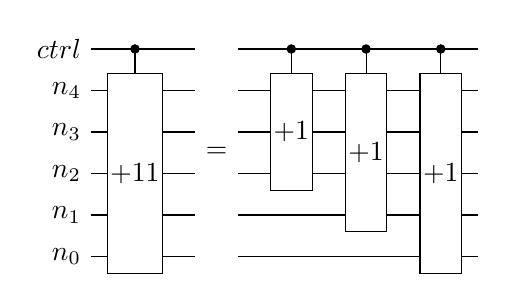
\begin{tikzpicture}[scale=1.000000,x=1pt,y=1pt]
\filldraw[color=white] (0.000000, -7.500000) rectangle (140.000000, 82.500000);
% Drawing wires
% Line 1: ctrl W ctrl
\draw[color=black] (0.000000,75.000000) -- (140.000000,75.000000);
\draw[color=black] (0.000000,75.000000) node[left] {$ctrl$};
% Line 2: n4 W n_4
\draw[color=black] (0.000000,60.000000) -- (140.000000,60.000000);
\draw[color=black] (0.000000,60.000000) node[left] {$n_4$};
% Line 3: n3 W n_3
\draw[color=black] (0.000000,45.000000) -- (140.000000,45.000000);
\draw[color=black] (0.000000,45.000000) node[left] {$n_3$};
% Line 4: n2 W n_2
\draw[color=black] (0.000000,30.000000) -- (140.000000,30.000000);
\draw[color=black] (0.000000,30.000000) node[left] {$n_2$};
% Line 5: n1 W n_1
\draw[color=black] (0.000000,15.000000) -- (140.000000,15.000000);
\draw[color=black] (0.000000,15.000000) node[left] {$n_1$};
% Line 6: n0 W n_0
\draw[color=black] (0.000000,0.000000) -- (140.000000,0.000000);
\draw[color=black] (0.000000,0.000000) node[left] {$n_0$};
% Done with wires; drawing gates
% Line 8: n4 n3 n2 n1 n0 G width=20 $+11$ ctrl
\draw (16.000000,75.000000) -- (16.000000,0.000000);
\begin{scope}
\draw[fill=white] (16.000000, 30.000000) +(-45.000000:14.142136pt and 50.911688pt) -- +(45.000000:14.142136pt and 50.911688pt) -- +(135.000000:14.142136pt and 50.911688pt) -- +(225.000000:14.142136pt and 50.911688pt) -- cycle;
\clip (16.000000, 30.000000) +(-45.000000:14.142136pt and 50.911688pt) -- +(45.000000:14.142136pt and 50.911688pt) -- +(135.000000:14.142136pt and 50.911688pt) -- +(225.000000:14.142136pt and 50.911688pt) -- cycle;
\draw (16.000000, 30.000000) node {$+11$};
\end{scope}
\filldraw (16.000000, 75.000000) circle(1.500000pt);
% Line 10: =
\draw[fill=white,color=white] (38.000000, -6.000000) rectangle (53.000000, 81.000000);
\draw (45.500000, 37.500000) node {$=$};
% Line 12: n4 n3 n2 G width=15 $+1$ ctrl
\draw (72.500000,75.000000) -- (72.500000,30.000000);
\begin{scope}
\draw[fill=white] (72.500000, 45.000000) +(-45.000000:10.606602pt and 29.698485pt) -- +(45.000000:10.606602pt and 29.698485pt) -- +(135.000000:10.606602pt and 29.698485pt) -- +(225.000000:10.606602pt and 29.698485pt) -- cycle;
\clip (72.500000, 45.000000) +(-45.000000:10.606602pt and 29.698485pt) -- +(45.000000:10.606602pt and 29.698485pt) -- +(135.000000:10.606602pt and 29.698485pt) -- +(225.000000:10.606602pt and 29.698485pt) -- cycle;
\draw (72.500000, 45.000000) node {$+1$};
\end{scope}
\filldraw (72.500000, 75.000000) circle(1.500000pt);
% Line 13: n4 n3 n2 n1 G width=15 $+1$ ctrl
\draw (99.500000,75.000000) -- (99.500000,15.000000);
\begin{scope}
\draw[fill=white] (99.500000, 37.500000) +(-45.000000:10.606602pt and 40.305087pt) -- +(45.000000:10.606602pt and 40.305087pt) -- +(135.000000:10.606602pt and 40.305087pt) -- +(225.000000:10.606602pt and 40.305087pt) -- cycle;
\clip (99.500000, 37.500000) +(-45.000000:10.606602pt and 40.305087pt) -- +(45.000000:10.606602pt and 40.305087pt) -- +(135.000000:10.606602pt and 40.305087pt) -- +(225.000000:10.606602pt and 40.305087pt) -- cycle;
\draw (99.500000, 37.500000) node {$+1$};
\end{scope}
\filldraw (99.500000, 75.000000) circle(1.500000pt);
% Line 14: n4 n3 n2 n1 n0 G width=15 $+1$ ctrl
\draw (126.500000,75.000000) -- (126.500000,0.000000);
\begin{scope}
\draw[fill=white] (126.500000, 30.000000) +(-45.000000:10.606602pt and 50.911688pt) -- +(45.000000:10.606602pt and 50.911688pt) -- +(135.000000:10.606602pt and 50.911688pt) -- +(225.000000:10.606602pt and 50.911688pt) -- cycle;
\clip (126.500000, 30.000000) +(-45.000000:10.606602pt and 50.911688pt) -- +(45.000000:10.606602pt and 50.911688pt) -- +(135.000000:10.606602pt and 50.911688pt) -- +(225.000000:10.606602pt and 50.911688pt) -- cycle;
\draw (126.500000, 30.000000) node {$+1$};
\end{scope}
\filldraw (126.500000, 75.000000) circle(1.500000pt);
% Done with gates; drawing ending labels
% Done with ending labels; drawing cut lines and comments
% Done with comments
\end{tikzpicture}

    \caption{
        \textbf{Addition via Incrementers} 
        An implementation of addition by a classical value ($11$) (mod $32$) using a series of incrementers is shown.
        An incrementer applied onto a register excluding the least-significant qubit implements a bit-shifted incrementer.
        This effectively increases the value of the register by $2$.
        Addition by the classical value $11$ can be constructed by bit-shifted incrementers adding the values $+8$, $+2$, and $+1$.
        Subtraction by the same value can be achieved by applying Pauli-X gates on each qubit before and after the operation.
    }
    \label{fig:addition-via-incrementers}
\end{figure}


However, an incrementer circuit can also be used to perform addition by a power of $2$ by acting on only the most-significant qubits.
For example, adding the value $8$ can be achieved using an incrementer circuit that treats the $4^{th}$ least significant qubit as the least significant qubit in the incrementer circuit and disregards the $3$ lesser qubits.
A circuit adding any classical value can then be constructed based on the binary representation of the classical number.
A circuit diagram for this construction is shown in Figure \ref{fig:addition-via-incrementers}.
The cost of this construction would require $N$ incrementer circuits requiring $4 \sum_{i=0}^{N - 2} N - i - 1$ T gates in total and $N - 1$ clean ancillae.

Since we are performing modular addition, the same result can also be achieved by subtracting the value $2^N - m$.
As an example, if the classical value is $31$ and $N = 5$, then this can be accomplished using a single decrementer circuit which can be constructed by conjugating an incrementer circuit with Pauli X gates acting on the qubits encoding $\ket{n}$.
The cost of these two methods can be classically determined and the more favorable option can be chosen during compilation.
The upper bound for the number of T gates, regardless of the classical value being added, is $N^2 + N$.
\ws{This scaling was determined numerically, but i think it shouldn't be hard to derive.}


\begin{figure}
    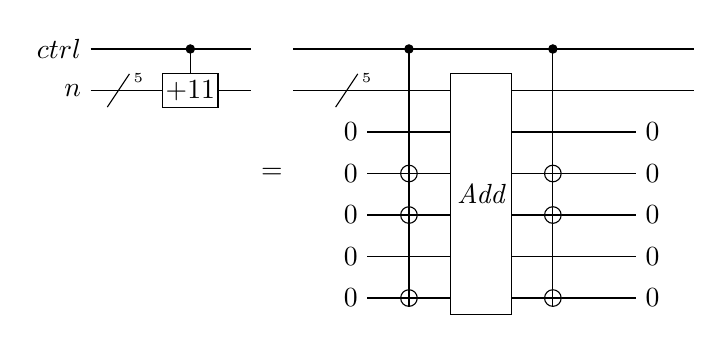
\begin{tikzpicture}[scale=1.000000,x=1pt,y=1pt]
\filldraw[color=white] (0.000000, -7.500000) rectangle (218.000000, 97.500000);
% Drawing wires
% Line 1: ctrl W ctrl
\draw[color=black] (0.000000,90.000000) -- (218.000000,90.000000);
\draw[color=black] (0.000000,90.000000) node[left] {$ctrl$};
% Line 2: n W n
\draw[color=black] (0.000000,75.000000) -- (218.000000,75.000000);
\draw[color=black] (0.000000,75.000000) node[left] {$n$};
% Line 3: m4 W 0 0
\draw[color=black] (92.500000,60.000000) -- (204.500000,60.000000);
% Line 4: m3 W 0 0
\draw[color=black] (92.500000,45.000000) -- (204.500000,45.000000);
% Line 5: m2 W 0 0
\draw[color=black] (92.500000,30.000000) -- (204.500000,30.000000);
% Line 6: m1 W 0 0
\draw[color=black] (92.500000,15.000000) -- (204.500000,15.000000);
% Line 7: m0 W 0 0
\draw[color=black] (92.500000,0.000000) -- (204.500000,0.000000);
% Done with wires; drawing gates
% Line 9: n / ^5
\draw (6.000000, 69.000000) -- (14.000000, 81.000000);
\draw (12.000000, 78.000000) node[right] {$\scriptstyle{^5}$};
% Line 11: n G width=20 $+11$ ctrl
\draw (36.000000,90.000000) -- (36.000000,75.000000);
\begin{scope}
\draw[fill=white] (36.000000, 75.000000) +(-45.000000:14.142136pt and 8.485281pt) -- +(45.000000:14.142136pt and 8.485281pt) -- +(135.000000:14.142136pt and 8.485281pt) -- +(225.000000:14.142136pt and 8.485281pt) -- cycle;
\clip (36.000000, 75.000000) +(-45.000000:14.142136pt and 8.485281pt) -- +(45.000000:14.142136pt and 8.485281pt) -- +(135.000000:14.142136pt and 8.485281pt) -- +(225.000000:14.142136pt and 8.485281pt) -- cycle;
\draw (36.000000, 75.000000) node {$+11$};
\end{scope}
\filldraw (36.000000, 90.000000) circle(1.500000pt);
% Line 13: =
\draw[fill=white,color=white] (58.000000, -6.000000) rectangle (73.000000, 96.000000);
\draw (65.500000, 45.000000) node {$=$};
% Line 15: n / ^5
\draw (88.500000, 69.000000) -- (96.500000, 81.000000);
\draw (94.500000, 78.000000) node[right] {$\scriptstyle{^5}$};
% Line 17: m4 START
\draw[color=black] (100.000000,60.000000) node[fill=white,left,minimum height=15.000000pt,minimum width=15.000000pt,inner sep=0pt] {\phantom{$0$}};
\draw[color=black] (100.000000,60.000000) node[left] {$0$};
% Line 18: m3 START
\draw[color=black] (100.000000,45.000000) node[fill=white,left,minimum height=15.000000pt,minimum width=15.000000pt,inner sep=0pt] {\phantom{$0$}};
\draw[color=black] (100.000000,45.000000) node[left] {$0$};
% Line 19: m2 START
\draw[color=black] (100.000000,30.000000) node[fill=white,left,minimum height=15.000000pt,minimum width=15.000000pt,inner sep=0pt] {\phantom{$0$}};
\draw[color=black] (100.000000,30.000000) node[left] {$0$};
% Line 20: m1 START
\draw[color=black] (100.000000,15.000000) node[fill=white,left,minimum height=15.000000pt,minimum width=15.000000pt,inner sep=0pt] {\phantom{$0$}};
\draw[color=black] (100.000000,15.000000) node[left] {$0$};
% Line 21: m0 START
\draw[color=black] (100.000000,0.000000) node[fill=white,left,minimum height=15.000000pt,minimum width=15.000000pt,inner sep=0pt] {\phantom{$0$}};
\draw[color=black] (100.000000,0.000000) node[left] {$0$};
% Line 22: ctrl +m3 +m2 +m0
\draw (115.000000,90.000000) -- (115.000000,0.000000);
\filldraw (115.000000, 90.000000) circle(1.500000pt);
\begin{scope}
\draw[fill=white] (115.000000, 45.000000) circle(3.000000pt);
\clip (115.000000, 45.000000) circle(3.000000pt);
\draw (112.000000, 45.000000) -- (118.000000, 45.000000);
\draw (115.000000, 42.000000) -- (115.000000, 48.000000);
\end{scope}
\begin{scope}
\draw[fill=white] (115.000000, 30.000000) circle(3.000000pt);
\clip (115.000000, 30.000000) circle(3.000000pt);
\draw (112.000000, 30.000000) -- (118.000000, 30.000000);
\draw (115.000000, 27.000000) -- (115.000000, 33.000000);
\end{scope}
\begin{scope}
\draw[fill=white] (115.000000, 0.000000) circle(3.000000pt);
\clip (115.000000, 0.000000) circle(3.000000pt);
\draw (112.000000, 0.000000) -- (118.000000, 0.000000);
\draw (115.000000, -3.000000) -- (115.000000, 3.000000);
\end{scope}
% Line 23: n m4 m3 m2 m1 m0 G width=22 $\textit{Add}$
\draw (141.000000,75.000000) -- (141.000000,0.000000);
\begin{scope}
\draw[fill=white] (141.000000, 37.500000) +(-45.000000:15.556349pt and 61.518290pt) -- +(45.000000:15.556349pt and 61.518290pt) -- +(135.000000:15.556349pt and 61.518290pt) -- +(225.000000:15.556349pt and 61.518290pt) -- cycle;
\clip (141.000000, 37.500000) +(-45.000000:15.556349pt and 61.518290pt) -- +(45.000000:15.556349pt and 61.518290pt) -- +(135.000000:15.556349pt and 61.518290pt) -- +(225.000000:15.556349pt and 61.518290pt) -- cycle;
\draw (141.000000, 37.500000) node {$\textit{Add}$};
\end{scope}
% Line 24: ctrl +m3 +m2 +m0
\draw (167.000000,90.000000) -- (167.000000,0.000000);
\filldraw (167.000000, 90.000000) circle(1.500000pt);
\begin{scope}
\draw[fill=white] (167.000000, 45.000000) circle(3.000000pt);
\clip (167.000000, 45.000000) circle(3.000000pt);
\draw (164.000000, 45.000000) -- (170.000000, 45.000000);
\draw (167.000000, 42.000000) -- (167.000000, 48.000000);
\end{scope}
\begin{scope}
\draw[fill=white] (167.000000, 30.000000) circle(3.000000pt);
\clip (167.000000, 30.000000) circle(3.000000pt);
\draw (164.000000, 30.000000) -- (170.000000, 30.000000);
\draw (167.000000, 27.000000) -- (167.000000, 33.000000);
\end{scope}
\begin{scope}
\draw[fill=white] (167.000000, 0.000000) circle(3.000000pt);
\clip (167.000000, 0.000000) circle(3.000000pt);
\draw (164.000000, 0.000000) -- (170.000000, 0.000000);
\draw (167.000000, -3.000000) -- (167.000000, 3.000000);
\end{scope}
% Line 25: m4 LABEL
% Line 26: m4 END
\draw[color=black] (197.000000,60.000000) node[fill=white,right,minimum height=15.000000pt,minimum width=15.000000pt,inner sep=0pt] {\phantom{$0$}};
\draw[color=black] (197.000000,60.000000) node[right] {$0$};
% Line 27: m3 END
\draw[color=black] (197.000000,45.000000) node[fill=white,right,minimum height=15.000000pt,minimum width=15.000000pt,inner sep=0pt] {\phantom{$0$}};
\draw[color=black] (197.000000,45.000000) node[right] {$0$};
% Line 28: m2 END
\draw[color=black] (197.000000,30.000000) node[fill=white,right,minimum height=15.000000pt,minimum width=15.000000pt,inner sep=0pt] {\phantom{$0$}};
\draw[color=black] (197.000000,30.000000) node[right] {$0$};
% Line 29: m1 END
\draw[color=black] (197.000000,15.000000) node[fill=white,right,minimum height=15.000000pt,minimum width=15.000000pt,inner sep=0pt] {\phantom{$0$}};
\draw[color=black] (197.000000,15.000000) node[right] {$0$};
% Line 30: m0 END
\draw[color=black] (197.000000,0.000000) node[fill=white,right,minimum height=15.000000pt,minimum width=15.000000pt,inner sep=0pt] {\phantom{$0$}};
\draw[color=black] (197.000000,0.000000) node[right] {$0$};
% Done with gates; drawing ending labels
% Done with ending labels; drawing cut lines and comments
% Done with comments
\end{tikzpicture}

    \caption{
        \textbf{Time-Efficient Controlled Addition of $11$}
        Increasing the value of a quantum register by a known classical value can be implemented using clean ancillae and an uncontrolled quantum addition circuit.
        The known classical value is loaded into a clean ancilla register using a series of CNOT gates corresponding to the binary representation of the classical value.
        Then an uncontrolled quantum addition circuit is applied to the two registers.
        Finally, the loading of the classical value is uncomputed.
    }
    \label{fig:addition-gate-efficient}
\end{figure}

Another option is to first load the classical value into an clean ancilla register, controlled on the control qubit, perform \textit{uncontrolled} (modular) addition of the two quantum registers, then ``unload'' the classical value.
If the control is off, then the classical value is not loaded and the uncontrolled addition simply adds the value $0$ and leaves the original register unchanged.
An example diagram for this construction depicting adding the value $m = 11$ to a register with $N = 5$ qubits is shown in Figure \ref{fig:addition-gate-efficient}.

The loading (and unloading) of the classical value only requires CNOTs and therefore does not contribute any non-Clifford resouces, but it does require $N$ clean ancillae.
However, if the $p$ least significant bits of $m$ are zero, then only $N - p$ qubits are required to load $m$ and the $p$ least-significant qubits of $N$ can be omitted from the addition.
Uncontrolled addition of two registers can be performed using $4(N-1)$ T gates and $N - 1$ clean ancillae using the construction for addition shown in Figure 1 of \cite{gidney2018halving}.
Therefore, in total, this compilation will require $4(N - p - 1)$ T gates and $2(N - p) - 1$ clean ancillae.

When $m$ is a power of $2$, then compilation using incrementer circuits uses the same number of T gates, but fewer clean ancillae.
When $m$ is not a power of $2$, then the compilation using uncontrolled quantum addition uses fewer T gates (at the expense of more clean ancillae).
Since $m$ is known during compilation, an implementation can be chosen that results in the fewest required resources.

\begin{figure*}
    \centering
    \includegraphics[width=12cm]{figures/ctrl-add-11-qubit-efficient.pdf}
    \caption{
        \textbf{Space-Efficient Controlled Addition of 11}
        An implementation for increasing the value of a register by a known classical value is shown for the case when the known value is $11$ and the number of qubits in the register is $5$.
        The binary representation of $11$ is $01011$ with the left-most bit being the most-significant.
        The values of these $M$ classical bits can be propagated into the control structure of the controlled quantum addition.
        If the value of the $i^\text{th}$ bit of $M$ is $0$ ($1$), the corresponding control in the circuit is controlled on the $\ket{1}$  ($\ket{0}$) state.
    }
    \label{fig:addition-qubit-efficient-11}
\end{figure*}

\begin{figure}
    \centering
    \includegraphics[width=8cm]{figures/ctrl-add-12-qubit-efficient.pdf}
    \caption{
        \textbf{Space-Efficient Controlled Addition of 12} 
        An implementation for increasing the value of a register by a known classical value is shown for the case when the known value is $12$ ($01100$ in binary) and the number of qubits in the register is $5$.
        When the least-significant bits of $M$ are $0$, the circuit can be bit-shifted, resulting in a lower cost implementation.
        In this case, the two least-significant bits are $0$, so the circuit can be bit-shifted twice.
    }
    \label{fig:addition-qubit-efficient-12}
\end{figure}

Another implementation can be chosen to reduce the number of clean ancillae, which uses the classical information about $m$ to modify the circuit for \textit{controlled} quantum addition.
Controlled addition of two registers can be performed using $4(2N - 3)$ T gates and $2N - 1$ clean ancillae using the construction for addition shown in Figure 4 of \cite{gidney2018halving}.
This circuit can be modified by propagating the classical information about the binary encoding of $m$ into the control structure of the adder circuit, thereby reducing the number of clean ancillae by $N$.
An example diagram showing this propagation in the case where $m = 11$ and $N = 5$ is shown in Figure \ref{fig:addition-qubit-efficient-11}.

Similarly, if the $p$ least-significant bits of $m$ are known to be zero, the addition can be performed beginning with the first non-zero bit of $m$.
An example circuit diagram for the case where $m=12$ ($01100$ in binary) and $N = 5$ is shown in Figure \ref{fig:addition-qubit-efficient-12}.
If the $p$ least significant bits of $m$ are zero, then this circuit uses $4(2(N - p) - 3)$ T gates and $N - p - 1$ clean ancillae.
Since this work primarily focuses on reducing the number of T gates, the quantum resource estimates quoted in this work do not utilize this strategy.

\section{Uniformly Controlled Rotations}
\label{sec:multiplexed-rotations}

Implementing a series of uniformly controlled rotations is a common subroutine used in this work.
In this section, we discuss the cost and explicit circuit compilation for a series of uniformly controlled rotations around the same axis (but different angles) are applied on the same qubit:
\begin{equation}
    \sum_{l=0}^{L - 1} \ket{l} \ket{\phi} \rightarrow \sum_{l=0}^{L - 1} \ket{l} R_a (\alpha_l) \ket{\phi}
\end{equation}

Möttönen et. al \cite{mottonen2004transformation}, provide a construction for \textit{uncontrolled} uniformly controlled rotations.
This construction is only defined when the number of rotations ($L$) is explicitly a power of $2$, however, if fewer rotations are required, then this can be achieved by padding with zero-angle rotations.

In this construction, the rotation angles are classically preprocessed based on the Gray code (Eq. 3 of \cite{mottonen2004transformation}):
\begin{equation}
    \begin{bmatrix}
        \theta_{0} \\
        \theta_{1} \\
        \vdots \\
        \theta_{L - 1}
    \end{bmatrix} = M \begin{bmatrix}
        \alpha_{0} \\
        \alpha_{1} \\
        \vdots \\
        \alpha_{L - 1}
    \end{bmatrix}
\end{equation}
where $M$ is a matrix transformation defined by:
\begin{equation}
    M_{i, j} = L^{-1} (-1)^{b_{j} . g_{i}}
\end{equation}
where $b_j$ is the binary representation of the integer $j$, $g_i$ is the Gray code representation of the integer $i$, and $b_{j} . g_{i}$ is the bitwise inner product of $b_{j}$ and $g_{i}$.

\begin{figure*}
    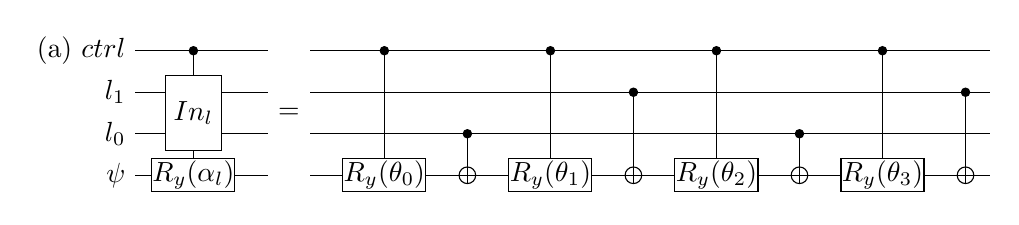
\begin{tikzpicture}[scale=1.000000,x=1pt,y=1pt]
\filldraw[color=white] (0.000000, -7.500000) rectangle (309.000000, 52.500000);
% Drawing wires
% Line 1: ctrl W \text{(a) }ctrl
\draw[color=black] (0.000000,45.000000) -- (309.000000,45.000000);
\draw[color=black] (0.000000,45.000000) node[left] {$\text{(a) }ctrl$};
% Line 2: l1 W l_1
\draw[color=black] (0.000000,30.000000) -- (309.000000,30.000000);
\draw[color=black] (0.000000,30.000000) node[left] {$l_1$};
% Line 3: l0 W l_0
\draw[color=black] (0.000000,15.000000) -- (309.000000,15.000000);
\draw[color=black] (0.000000,15.000000) node[left] {$l_0$};
% Line 4: sys W \psi
\draw[color=black] (0.000000,0.000000) -- (309.000000,0.000000);
\draw[color=black] (0.000000,0.000000) node[left] {$\psi$};
% Done with wires; drawing gates
% Line 6: l1 l0 G:width=20 $In_l$ sys G:width=30 $R_y (\alpha_l)$ ctrl
\draw (21.000000,45.000000) -- (21.000000,0.000000);
\begin{scope}
\draw[fill=white] (21.000000, 22.500000) +(-45.000000:14.142136pt and 19.091883pt) -- +(45.000000:14.142136pt and 19.091883pt) -- +(135.000000:14.142136pt and 19.091883pt) -- +(225.000000:14.142136pt and 19.091883pt) -- cycle;
\clip (21.000000, 22.500000) +(-45.000000:14.142136pt and 19.091883pt) -- +(45.000000:14.142136pt and 19.091883pt) -- +(135.000000:14.142136pt and 19.091883pt) -- +(225.000000:14.142136pt and 19.091883pt) -- cycle;
\draw (21.000000, 22.500000) node {$In_l$};
\end{scope}
\begin{scope}
\draw[fill=white] (21.000000, -0.000000) +(-45.000000:21.213203pt and 8.485281pt) -- +(45.000000:21.213203pt and 8.485281pt) -- +(135.000000:21.213203pt and 8.485281pt) -- +(225.000000:21.213203pt and 8.485281pt) -- cycle;
\clip (21.000000, -0.000000) +(-45.000000:21.213203pt and 8.485281pt) -- +(45.000000:21.213203pt and 8.485281pt) -- +(135.000000:21.213203pt and 8.485281pt) -- +(225.000000:21.213203pt and 8.485281pt) -- cycle;
\draw (21.000000, -0.000000) node {$R_y (\alpha_l)$};
\end{scope}
\filldraw (21.000000, 45.000000) circle(1.500000pt);
% Line 8: =
\draw[fill=white,color=white] (48.000000, -6.000000) rectangle (63.000000, 51.000000);
\draw (55.500000, 22.500000) node {$=$};
% Line 10: sys G width=30 $R_y (\theta_0)$ ctrl
\draw (90.000000,45.000000) -- (90.000000,0.000000);
\begin{scope}
\draw[fill=white] (90.000000, -0.000000) +(-45.000000:21.213203pt and 8.485281pt) -- +(45.000000:21.213203pt and 8.485281pt) -- +(135.000000:21.213203pt and 8.485281pt) -- +(225.000000:21.213203pt and 8.485281pt) -- cycle;
\clip (90.000000, -0.000000) +(-45.000000:21.213203pt and 8.485281pt) -- +(45.000000:21.213203pt and 8.485281pt) -- +(135.000000:21.213203pt and 8.485281pt) -- +(225.000000:21.213203pt and 8.485281pt) -- cycle;
\draw (90.000000, -0.000000) node {$R_y (\theta_0)$};
\end{scope}
\filldraw (90.000000, 45.000000) circle(1.500000pt);
% Line 11: +sys l0
\draw (120.000000,15.000000) -- (120.000000,0.000000);
\begin{scope}
\draw[fill=white] (120.000000, 0.000000) circle(3.000000pt);
\clip (120.000000, 0.000000) circle(3.000000pt);
\draw (117.000000, 0.000000) -- (123.000000, 0.000000);
\draw (120.000000, -3.000000) -- (120.000000, 3.000000);
\end{scope}
\filldraw (120.000000, 15.000000) circle(1.500000pt);
% Line 12: sys G width=30 $R_y (\theta_1)$ ctrl
\draw (150.000000,45.000000) -- (150.000000,0.000000);
\begin{scope}
\draw[fill=white] (150.000000, -0.000000) +(-45.000000:21.213203pt and 8.485281pt) -- +(45.000000:21.213203pt and 8.485281pt) -- +(135.000000:21.213203pt and 8.485281pt) -- +(225.000000:21.213203pt and 8.485281pt) -- cycle;
\clip (150.000000, -0.000000) +(-45.000000:21.213203pt and 8.485281pt) -- +(45.000000:21.213203pt and 8.485281pt) -- +(135.000000:21.213203pt and 8.485281pt) -- +(225.000000:21.213203pt and 8.485281pt) -- cycle;
\draw (150.000000, -0.000000) node {$R_y (\theta_1)$};
\end{scope}
\filldraw (150.000000, 45.000000) circle(1.500000pt);
% Line 13: +sys l1
\draw (180.000000,30.000000) -- (180.000000,0.000000);
\begin{scope}
\draw[fill=white] (180.000000, 0.000000) circle(3.000000pt);
\clip (180.000000, 0.000000) circle(3.000000pt);
\draw (177.000000, 0.000000) -- (183.000000, 0.000000);
\draw (180.000000, -3.000000) -- (180.000000, 3.000000);
\end{scope}
\filldraw (180.000000, 30.000000) circle(1.500000pt);
% Line 14: sys G width=30 $R_y (\theta_2)$ ctrl
\draw (210.000000,45.000000) -- (210.000000,0.000000);
\begin{scope}
\draw[fill=white] (210.000000, -0.000000) +(-45.000000:21.213203pt and 8.485281pt) -- +(45.000000:21.213203pt and 8.485281pt) -- +(135.000000:21.213203pt and 8.485281pt) -- +(225.000000:21.213203pt and 8.485281pt) -- cycle;
\clip (210.000000, -0.000000) +(-45.000000:21.213203pt and 8.485281pt) -- +(45.000000:21.213203pt and 8.485281pt) -- +(135.000000:21.213203pt and 8.485281pt) -- +(225.000000:21.213203pt and 8.485281pt) -- cycle;
\draw (210.000000, -0.000000) node {$R_y (\theta_2)$};
\end{scope}
\filldraw (210.000000, 45.000000) circle(1.500000pt);
% Line 15: +sys l0
\draw (240.000000,15.000000) -- (240.000000,0.000000);
\begin{scope}
\draw[fill=white] (240.000000, 0.000000) circle(3.000000pt);
\clip (240.000000, 0.000000) circle(3.000000pt);
\draw (237.000000, 0.000000) -- (243.000000, 0.000000);
\draw (240.000000, -3.000000) -- (240.000000, 3.000000);
\end{scope}
\filldraw (240.000000, 15.000000) circle(1.500000pt);
% Line 16: sys G width=30 $R_y (\theta_3)$ ctrl
\draw (270.000000,45.000000) -- (270.000000,0.000000);
\begin{scope}
\draw[fill=white] (270.000000, -0.000000) +(-45.000000:21.213203pt and 8.485281pt) -- +(45.000000:21.213203pt and 8.485281pt) -- +(135.000000:21.213203pt and 8.485281pt) -- +(225.000000:21.213203pt and 8.485281pt) -- cycle;
\clip (270.000000, -0.000000) +(-45.000000:21.213203pt and 8.485281pt) -- +(45.000000:21.213203pt and 8.485281pt) -- +(135.000000:21.213203pt and 8.485281pt) -- +(225.000000:21.213203pt and 8.485281pt) -- cycle;
\draw (270.000000, -0.000000) node {$R_y (\theta_3)$};
\end{scope}
\filldraw (270.000000, 45.000000) circle(1.500000pt);
% Line 17: +sys l1
\draw (300.000000,30.000000) -- (300.000000,0.000000);
\begin{scope}
\draw[fill=white] (300.000000, 0.000000) circle(3.000000pt);
\clip (300.000000, 0.000000) circle(3.000000pt);
\draw (297.000000, 0.000000) -- (303.000000, 0.000000);
\draw (300.000000, -3.000000) -- (300.000000, 3.000000);
\end{scope}
\filldraw (300.000000, 30.000000) circle(1.500000pt);
% Done with gates; drawing ending labels
% Done with ending labels; drawing cut lines and comments
% Done with comments
\end{tikzpicture}

    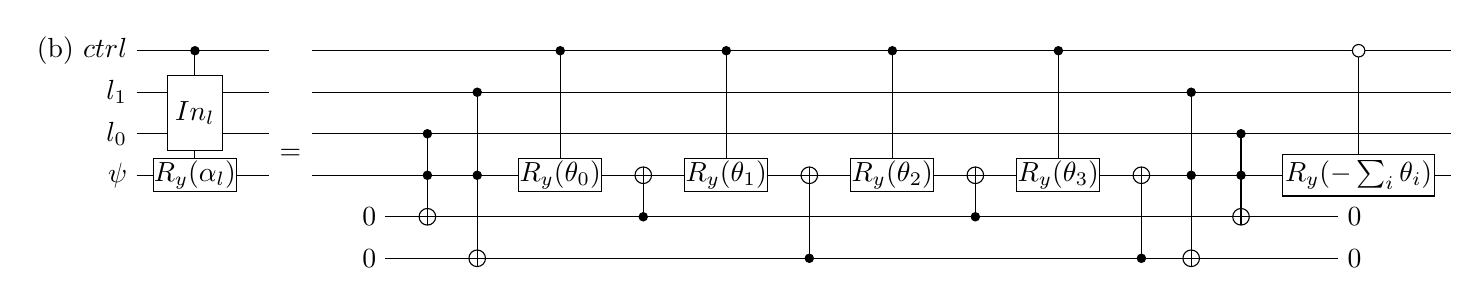
\begin{tikzpicture}[scale=1.000000,x=1pt,y=1pt]
\filldraw[color=white] (0.000000, -7.500000) rectangle (475.000000, 82.500000);
% Drawing wires
% Line 1: ctrl W \text{(b) }ctrl
\draw[color=black] (0.000000,75.000000) -- (475.000000,75.000000);
\draw[color=black] (0.000000,75.000000) node[left] {$\text{(b) }ctrl$};
% Line 2: l1 W l_1
\draw[color=black] (0.000000,60.000000) -- (475.000000,60.000000);
\draw[color=black] (0.000000,60.000000) node[left] {$l_1$};
% Line 3: l0 W l_0
\draw[color=black] (0.000000,45.000000) -- (475.000000,45.000000);
\draw[color=black] (0.000000,45.000000) node[left] {$l_0$};
% Line 4: sys W \psi
\draw[color=black] (0.000000,30.000000) -- (475.000000,30.000000);
\draw[color=black] (0.000000,30.000000) node[left] {$\psi$};
% Line 5: c0 W 0 0
\draw[color=black] (82.500000,15.000000) -- (441.500000,15.000000);
% Line 6: c1 W 0 0
\draw[color=black] (82.500000,0.000000) -- (441.500000,0.000000);
% Done with wires; drawing gates
% Line 8: sys G:width=30 $R_y (\alpha_l)$ l1 l0 G:width=20 $In_l$ ctrl
\draw (21.000000,75.000000) -- (21.000000,30.000000);
\begin{scope}
\draw[fill=white] (21.000000, 30.000000) +(-45.000000:21.213203pt and 8.485281pt) -- +(45.000000:21.213203pt and 8.485281pt) -- +(135.000000:21.213203pt and 8.485281pt) -- +(225.000000:21.213203pt and 8.485281pt) -- cycle;
\clip (21.000000, 30.000000) +(-45.000000:21.213203pt and 8.485281pt) -- +(45.000000:21.213203pt and 8.485281pt) -- +(135.000000:21.213203pt and 8.485281pt) -- +(225.000000:21.213203pt and 8.485281pt) -- cycle;
\draw (21.000000, 30.000000) node {$R_y (\alpha_l)$};
\end{scope}
\begin{scope}
\draw[fill=white] (21.000000, 52.500000) +(-45.000000:14.142136pt and 19.091883pt) -- +(45.000000:14.142136pt and 19.091883pt) -- +(135.000000:14.142136pt and 19.091883pt) -- +(225.000000:14.142136pt and 19.091883pt) -- cycle;
\clip (21.000000, 52.500000) +(-45.000000:14.142136pt and 19.091883pt) -- +(45.000000:14.142136pt and 19.091883pt) -- +(135.000000:14.142136pt and 19.091883pt) -- +(225.000000:14.142136pt and 19.091883pt) -- cycle;
\draw (21.000000, 52.500000) node {$In_l$};
\end{scope}
\filldraw (21.000000, 75.000000) circle(1.500000pt);
% Line 10: =
\draw[fill=white,color=white] (48.000000, -6.000000) rectangle (63.000000, 81.000000);
\draw (55.500000, 37.500000) node {$=$};
% Line 12: c0 c1 START
\draw[color=black] (90.000000,15.000000) node[fill=white,left,minimum height=15.000000pt,minimum width=15.000000pt,inner sep=0pt] {\phantom{$0$}};
\draw[color=black] (90.000000,15.000000) node[left] {$0$};
\draw[color=black] (90.000000,0.000000) node[fill=white,left,minimum height=15.000000pt,minimum width=15.000000pt,inner sep=0pt] {\phantom{$0$}};
\draw[color=black] (90.000000,0.000000) node[left] {$0$};
% Line 13: +c0 sys l0
\draw (105.000000,45.000000) -- (105.000000,15.000000);
\begin{scope}
\draw[fill=white] (105.000000, 15.000000) circle(3.000000pt);
\clip (105.000000, 15.000000) circle(3.000000pt);
\draw (102.000000, 15.000000) -- (108.000000, 15.000000);
\draw (105.000000, 12.000000) -- (105.000000, 18.000000);
\end{scope}
\filldraw (105.000000, 30.000000) circle(1.500000pt);
\filldraw (105.000000, 45.000000) circle(1.500000pt);
% Line 14: +c1 sys l1
\draw (123.000000,60.000000) -- (123.000000,0.000000);
\begin{scope}
\draw[fill=white] (123.000000, 0.000000) circle(3.000000pt);
\clip (123.000000, 0.000000) circle(3.000000pt);
\draw (120.000000, 0.000000) -- (126.000000, 0.000000);
\draw (123.000000, -3.000000) -- (123.000000, 3.000000);
\end{scope}
\filldraw (123.000000, 30.000000) circle(1.500000pt);
\filldraw (123.000000, 60.000000) circle(1.500000pt);
% Line 16: sys G width=30 $R_y (\theta_0)$ ctrl
\draw (153.000000,75.000000) -- (153.000000,30.000000);
\begin{scope}
\draw[fill=white] (153.000000, 30.000000) +(-45.000000:21.213203pt and 8.485281pt) -- +(45.000000:21.213203pt and 8.485281pt) -- +(135.000000:21.213203pt and 8.485281pt) -- +(225.000000:21.213203pt and 8.485281pt) -- cycle;
\clip (153.000000, 30.000000) +(-45.000000:21.213203pt and 8.485281pt) -- +(45.000000:21.213203pt and 8.485281pt) -- +(135.000000:21.213203pt and 8.485281pt) -- +(225.000000:21.213203pt and 8.485281pt) -- cycle;
\draw (153.000000, 30.000000) node {$R_y (\theta_0)$};
\end{scope}
\filldraw (153.000000, 75.000000) circle(1.500000pt);
% Line 17: +sys c0
\draw (183.000000,30.000000) -- (183.000000,15.000000);
\begin{scope}
\draw[fill=white] (183.000000, 30.000000) circle(3.000000pt);
\clip (183.000000, 30.000000) circle(3.000000pt);
\draw (180.000000, 30.000000) -- (186.000000, 30.000000);
\draw (183.000000, 27.000000) -- (183.000000, 33.000000);
\end{scope}
\filldraw (183.000000, 15.000000) circle(1.500000pt);
% Line 18: sys G width=30 $R_y (\theta_1)$ ctrl
\draw (213.000000,75.000000) -- (213.000000,30.000000);
\begin{scope}
\draw[fill=white] (213.000000, 30.000000) +(-45.000000:21.213203pt and 8.485281pt) -- +(45.000000:21.213203pt and 8.485281pt) -- +(135.000000:21.213203pt and 8.485281pt) -- +(225.000000:21.213203pt and 8.485281pt) -- cycle;
\clip (213.000000, 30.000000) +(-45.000000:21.213203pt and 8.485281pt) -- +(45.000000:21.213203pt and 8.485281pt) -- +(135.000000:21.213203pt and 8.485281pt) -- +(225.000000:21.213203pt and 8.485281pt) -- cycle;
\draw (213.000000, 30.000000) node {$R_y (\theta_1)$};
\end{scope}
\filldraw (213.000000, 75.000000) circle(1.500000pt);
% Line 19: +sys c1
\draw (243.000000,30.000000) -- (243.000000,0.000000);
\begin{scope}
\draw[fill=white] (243.000000, 30.000000) circle(3.000000pt);
\clip (243.000000, 30.000000) circle(3.000000pt);
\draw (240.000000, 30.000000) -- (246.000000, 30.000000);
\draw (243.000000, 27.000000) -- (243.000000, 33.000000);
\end{scope}
\filldraw (243.000000, 0.000000) circle(1.500000pt);
% Line 20: sys G width=30 $R_y (\theta_2)$ ctrl
\draw (273.000000,75.000000) -- (273.000000,30.000000);
\begin{scope}
\draw[fill=white] (273.000000, 30.000000) +(-45.000000:21.213203pt and 8.485281pt) -- +(45.000000:21.213203pt and 8.485281pt) -- +(135.000000:21.213203pt and 8.485281pt) -- +(225.000000:21.213203pt and 8.485281pt) -- cycle;
\clip (273.000000, 30.000000) +(-45.000000:21.213203pt and 8.485281pt) -- +(45.000000:21.213203pt and 8.485281pt) -- +(135.000000:21.213203pt and 8.485281pt) -- +(225.000000:21.213203pt and 8.485281pt) -- cycle;
\draw (273.000000, 30.000000) node {$R_y (\theta_2)$};
\end{scope}
\filldraw (273.000000, 75.000000) circle(1.500000pt);
% Line 21: +sys c0
\draw (303.000000,30.000000) -- (303.000000,15.000000);
\begin{scope}
\draw[fill=white] (303.000000, 30.000000) circle(3.000000pt);
\clip (303.000000, 30.000000) circle(3.000000pt);
\draw (300.000000, 30.000000) -- (306.000000, 30.000000);
\draw (303.000000, 27.000000) -- (303.000000, 33.000000);
\end{scope}
\filldraw (303.000000, 15.000000) circle(1.500000pt);
% Line 22: sys G width=30 $R_y (\theta_3)$ ctrl
\draw (333.000000,75.000000) -- (333.000000,30.000000);
\begin{scope}
\draw[fill=white] (333.000000, 30.000000) +(-45.000000:21.213203pt and 8.485281pt) -- +(45.000000:21.213203pt and 8.485281pt) -- +(135.000000:21.213203pt and 8.485281pt) -- +(225.000000:21.213203pt and 8.485281pt) -- cycle;
\clip (333.000000, 30.000000) +(-45.000000:21.213203pt and 8.485281pt) -- +(45.000000:21.213203pt and 8.485281pt) -- +(135.000000:21.213203pt and 8.485281pt) -- +(225.000000:21.213203pt and 8.485281pt) -- cycle;
\draw (333.000000, 30.000000) node {$R_y (\theta_3)$};
\end{scope}
\filldraw (333.000000, 75.000000) circle(1.500000pt);
% Line 23: +sys c1
\draw (363.000000,30.000000) -- (363.000000,0.000000);
\begin{scope}
\draw[fill=white] (363.000000, 30.000000) circle(3.000000pt);
\clip (363.000000, 30.000000) circle(3.000000pt);
\draw (360.000000, 30.000000) -- (366.000000, 30.000000);
\draw (363.000000, 27.000000) -- (363.000000, 33.000000);
\end{scope}
\filldraw (363.000000, 0.000000) circle(1.500000pt);
% Line 25: +c1 sys l1
\draw (381.000000,60.000000) -- (381.000000,0.000000);
\begin{scope}
\draw[fill=white] (381.000000, 0.000000) circle(3.000000pt);
\clip (381.000000, 0.000000) circle(3.000000pt);
\draw (378.000000, 0.000000) -- (384.000000, 0.000000);
\draw (381.000000, -3.000000) -- (381.000000, 3.000000);
\end{scope}
\filldraw (381.000000, 30.000000) circle(1.500000pt);
\filldraw (381.000000, 60.000000) circle(1.500000pt);
% Line 26: +c0 sys l0
\draw (399.000000,45.000000) -- (399.000000,15.000000);
\begin{scope}
\draw[fill=white] (399.000000, 15.000000) circle(3.000000pt);
\clip (399.000000, 15.000000) circle(3.000000pt);
\draw (396.000000, 15.000000) -- (402.000000, 15.000000);
\draw (399.000000, 12.000000) -- (399.000000, 18.000000);
\end{scope}
\filldraw (399.000000, 30.000000) circle(1.500000pt);
\filldraw (399.000000, 45.000000) circle(1.500000pt);
% Line 27: c0 c1 END
\draw[color=black] (434.000000,15.000000) node[fill=white,right,minimum height=15.000000pt,minimum width=15.000000pt,inner sep=0pt] {\phantom{$0$}};
\draw[color=black] (434.000000,15.000000) node[right] {$0$};
\draw[color=black] (434.000000,0.000000) node[fill=white,right,minimum height=15.000000pt,minimum width=15.000000pt,inner sep=0pt] {\phantom{$0$}};
\draw[color=black] (434.000000,0.000000) node[right] {$0$};
% Line 29: sys G:width=55:height=15 $R_y(-\sum_i \theta_i)$ -ctrl
\draw (441.500000,75.000000) -- (441.500000,30.000000);
\begin{scope}
\draw[fill=white] (441.500000, 30.000000) +(-45.000000:38.890873pt and 10.606602pt) -- +(45.000000:38.890873pt and 10.606602pt) -- +(135.000000:38.890873pt and 10.606602pt) -- +(225.000000:38.890873pt and 10.606602pt) -- cycle;
\clip (441.500000, 30.000000) +(-45.000000:38.890873pt and 10.606602pt) -- +(45.000000:38.890873pt and 10.606602pt) -- +(135.000000:38.890873pt and 10.606602pt) -- +(225.000000:38.890873pt and 10.606602pt) -- cycle;
\draw (441.500000, 30.000000) node {$R_y(-\sum_i \theta_i)$};
\end{scope}
\draw[fill=white] (441.500000, 75.000000) circle(2.250000pt);
% Done with gates; drawing ending labels
% Done with ending labels; drawing cut lines and comments
% Done with comments
\end{tikzpicture}

    \caption{
        \textbf{Controlled Uniformly Controlled Rotations}
        Two implementations for controlling a series of uniformly controlled rotations are shown.
        In (a), a naive implementation is shown which doubles the number of arbitrary rotations required.
        The implementation shown in (b) uses only one additional controlled rotation and $\log_2 L$ Toffoli gates, but requires $\log_2 L$ clean ancillae.
    }
    \label{fig:controlled-multiplexed-rotations}
\end{figure*}

However, in this work we require the use of a \textit{controlled} series of uniformly controlled rotations.
Naively, this can be implemented by controlling each of the arbitrary rotations in the construction given by Möttönen et al. \cite{mottonen2004transformation}.
An example circuit diagram for this construction is shown in subfigure \ref{fig:controlled-multiplexed-rotations}a.
Since each controlled rotation can be implemented by two uncontrolled rotations, this compilation strategy uses $2L$ uncontrolled arbitrary rotations.

An alternative approach which uses $4 \log_2 L$ T gates, $L + 3$ arbitrary rotations, and $\log_2 L$ clean ancillae is shown in subfigure \ref{fig:controlled-multiplexed-rotations}b.
In this construction, the temporary logical-AND of each qubit in the index register and the control qubit is computed using $\log_2 L$ Toffoli gates.
CNOTs from these clean ancillae then conjugate each of the arbitrary rotations which are left uncontrolled.
When the control is on, this fully recovers the construction given by Möttönen et. al.

However, when the control is off, the uncontrolled arbitrary rotations are still applied, resulting an undesired rotation of angle $\sum_{i} (\theta_i)$.
This undesired rotation can then be undone using one $0$-controlled rotation of angle $- \sum_{i} (\theta_i)$.

\section{Grover-Rudolph State Preparation}
\label{sec:grover-rudolph}

In this section, we will describe the Grover-Rudolph state-preparation routine \cite{grover2002creating} in the context that it is used in this work.
The Grover-Rudolph state-preparation algorithm constructs quantum circuits that prepare states of the form given by:
\begin{equation}
    \ket{0^{\otimes \lceil \log_2{L} \rceil}} \rightarrow_{\textit{Grover-Rudolph}} \sum_{l=0}^L \sqrt{p(l)} \ket{l}
\end{equation}
where $p(l)$ is a probability distribution along the different indices ($l$) with the constraint that $\sum_l p(l) = 1$.

In the context of block-encodings, preparing such probability distributions can be used to construct the $Prepare$ oracle:
\begin{equation}
    \ket{0^{\otimes \lceil \log_2{L} \rceil}} \rightarrow_{\textit{Prepare}} \sum_{l = 0}^{L-1} \sqrt{|\alpha_l| / \lambda_{ASP}} \ket{l}
\end{equation}
where the probability distribution is defined by the normalized magnitudes of the coefficients of the terms in the linear combination: $p(l) = |\alpha_l| / \lambda_{ASP}$.

The Grover-Rudolph algorithm works by sequentially summing up the probability distribution to the left and right of a given index and then performing a rotation controlled based on the current index.

For example, given the coefficients $\alpha_0$, $\alpha_1$, $\alpha_2$, and $\alpha_3$, the Grover-Rudolph algorithm proceeds as follows:
\begin{enumerate}
    \item Perform a Pauli-Y rotation on the top (left-most) qubit in the register by an angle: $\theta = 2 \cos^{-1}\big( \sqrt{\alpha_0 + \alpha_1} \big)$.
    \item Perform a Pauli-Y rotation on the second qubit in the register, controlled on the first qubit being in the state $\ket{0}$ by an angle: $\theta = 2 \cos^{-1}\big( \sqrt{\frac{\alpha_0}{\alpha_0 + \alpha_1}} \big)$
    \item Perform a Pauli-Y rotation on the second qubit in the register, controlled on the first qubit being in the state $\ket{1}$ by an angle: $\theta = 2 \cos^{-1}\big( \sqrt{\frac{\alpha_2}{\alpha_2 + \alpha_3}} \big)$
\end{enumerate}

The evolution of the quantum state is described by:
\begin{equation}
    \begin{split}
        \ket{00} &\rightarrow_{\textit{(i)}} \sqrt{\alpha_0 + \alpha_1} \ket{00} + \sqrt{\alpha_2 + \alpha_3} \ket{10} \\
        &\rightarrow_{\textit{(ii)}} \sqrt{\alpha_0} \ket{00} + \sqrt{\alpha_1} \ket{01} + \sqrt{\alpha_2 + \alpha_3} \ket{10} \\
        &\rightarrow_{\textit{(iii)}} \sqrt{\alpha_0} \ket{00} + \sqrt{\alpha_1} \ket{01} + \alpha_2 \ket{10} + \alpha_3 \ket{11}
    \end{split}
\end{equation}

In Figure \ref{fig:grover-rudolph} a, we show how implementing Grover-Rudolph can be viewed as a series of multiplexed rotations that sequentially act on the next qubit while indexing over the preceeding qubits in the register being prepared.
Prior works \cite{mottonen2004transformation, low2021halving} have shown that multiplexed rotations can be implemented more efficiently than other multiplexed operations by classically preprocessing the rotation angles. 
In Figure \ref{fig:grover-rudolph} b, we show how implementing Grover-Rudolph using the decomposition for multiplexed rotations of \cite{mottonen2004transformation} leads to requiring $L-1$ uncontrolled rotations when preparing $L$ coefficients.
\ws{This value of $L-1$ rotations is certainly true when $L$ is a power of 2. It's not clear that when some of the rotation angles are zero before the classical preprocessing that this cost will still be $L-1$ rotations and not the next highest power of 2.}

\begin{figure}
    \centering
    \includegraphics[width=16cm]{figures/grover-rudolph.pdf}
    % \includegraphics[width=16cm]{figures/grover-rudolph-4-qubits.pdf}
    \caption{
        \textbf{Grover-Rudolph Circuit Compilation.} 
        This figure shows an implementation of the Grover-Rudolph algorithm using multiplexed rotations when preparing 8 coefficients.
        The left subfigure shows the circuit diagram explicitly written as multiplexors, while the right subfigure shows the circuit when the multiplexed rotations are decomposed via \cite{mottonen2004transformation}.
        This circuit requires 7 rotations and the angles of the rotations are changed ($\theta_i \rightarrow \alpha_i$) based on classical preprocessing.
    }
    \label{fig:grover-rudolph}
\end{figure}

\section{Example}
\label{subsec:example}
%Step-by-step example (intention is to move this to an appendix)
Here, a contrived Hamiltonian is used to show the step-by-step procedure of LOBE. The example Hamiltonian, with a bosonic occupancy cutoff $\Omega = 3$, that will be used is 

\begin{equation}
    H = b_0^\dagger d_0(a_0^\dagger)^2 + 2 d_0^\dagger a_0^\dagger a_0+3 b_0^\dagger d_0^\dagger d_0
\end{equation}

\textbf{Step 1: Rescale Hamiltonian from bosonic terms:}
Via equation \ref{bose coeff rescale}, $\frac{1}{(\Omega + 1)^{K/2}} = \frac{1}{4}$ because $K = 2$ (there are at most 2 bosonic creation/annihilation terms, which in this case come from the first term). Now the Hamiltonian becomes 
\begin{equation}
    H^* = \frac{1}{4}H
\end{equation}

\textbf{Step 2: Rescale coefficients of Hamiltonian (assuming USP):} In order to load the Hamiltonian coefficients into the circuit via the $R_y$ gates in the \textit{coefficient} oracle, we need to ensure the coefficients are $\leq 1$. This is done via equation \ref{usp scale}. 
In this case, $L = 3$ since there are three terms, and $\alpha^* = 3$, the largest term coefficient. Thus, $\lambda_{usp} = 12$. Now, via \ref{Hbar scale}, the fully rescaled Hamiltonian is:
\begin{equation}
    \bar{H} = \frac{1}{48}b_0^\dagger d_0(a_0^\dagger)^2 + \frac{1}{24} d_0^\dagger a_0^\dagger a_0+\frac{1}{16} b_0^\dagger d_0^\dagger d_0
\end{equation}

\textbf{Step 3: Obtain the corresponding LOBE circuit:} In the style of figure \ref{fig:select-normal-ordering}, for this particular Hamiltonian, the three \textit{select} oracle unitaries: $U_{T_0}, U_{T_1}, U_{T_2}$ appear as:
\begin{figure}[h]
    \includegraphics[width = 0.7\linewidth]{figures/T0.png}
    \caption{\textit{Select} unitary $U_{T_0}$ that block-encodes $T_0 = \frac{1}{48}b_0^\dagger d_0(a_0^\dagger)^2$}
\end{figure}
\begin{figure}[h]
    \includegraphics[width = 0.7\linewidth]{figures/T1.png}
    \caption{\textit{Select} unitary $U_{T_1}$ that block-encodes $T_1 = \frac{1}{24}a_0^\dagger a_0 d_0^\dagger$}
\end{figure}
\begin{figure}[h]
    \includegraphics[width = 0.7\linewidth]{figures/T2.png}
    \caption{\textit{Select} unitary $U_{T_2}$ that block-encodes $T_2 = \frac{1}{16}b_0^\dagger d_0^\dagger d_0$}
\end{figure}

\textbf{Step 4: Count gates:} Using the notation in \ref{count gates not.}, the preceeding three unitaries have the following gate counts:

\begin{align}
    C_{U_{T_0}} &= (3, 1, 5, 5)\\
    C_{U_{T_1}} &= (4, 1, 5, 5)\\
    C_{U_{T_2}} &= (1, 1, 3, 3)
\end{align}
Thus, the total cost of the \textit{select} oracle is $C_{\textit{select}} = (8, 3, 13, 13)$. 

\textbf{Step 5: Post-process the eigenvalues:} After obtaining the full block-encoding of the Hamiltonian, the eigenvalues (which can be obtained via phase estimation) must be post-processed. This is because the eigenvalues of the block encoded Hamiltonian will correspond to $\bar{H}$, \textit{not} $H$ (the original problem Hamiltonian).
For this example, $\bar{H} = \frac{1}{48}H$, so if eigenvalues of the block Hamiltonian are obtained as $\bar{E}_i$, then $\bar{E_i} = \frac{1}{48}E_i$. Thus,
\begin{equation}
    E_i = 48\bar{E}_i
\end{equation}

\end{document}